\documentclass[12pt,openany]{book}

% -------------------- Packages --------------------
\usepackage[a4paper,margin=1in]{geometry}
\usepackage[T1]{fontenc}
\usepackage{lmodern}
\usepackage{amsmath,amssymb,amsthm,mathtools}
\usepackage{graphicx}
\usepackage{xurl}
\usepackage{float}
\usepackage{hyperref}
\usepackage{fancyhdr}
\usepackage{titlesec}
\usepackage{enumitem}
\usepackage{array}
\usepackage{booktabs,longtable}
\usepackage{textcomp}
\usepackage{listings}
\usepackage{imakeidx}
\usepackage{xcolor}
\usepackage{tikz}
\usepackage{placeins}
\usepackage{microtype}
\usetikzlibrary{arrows.meta,positioning,calc,shapes.geometric}
\DeclareUnicodeCharacter{20B9}{Rs.\ }
\DeclareUnicodeCharacter{00D7}{\(\times\)}
\DeclareUnicodeCharacter{00B2}{\textsuperscript{2}}
\DeclareUnicodeCharacter{2030}{\textperthousand{}}
\DeclareUnicodeCharacter{2013}{--}
\DeclareUnicodeCharacter{2014}{---}
\DeclareUnicodeCharacter{2191}{\(\uparrow\)}
\DeclareUnicodeCharacter{2192}{\(\rightarrow\)}
\DeclareUnicodeCharacter{2193}{\(\downarrow\)}
\DeclareUnicodeCharacter{2212}{\(-\)}
\DeclareUnicodeCharacter{2248}{\(\approx\)}
\DeclareUnicodeCharacter{2260}{\(\neq\)}
\DeclareUnicodeCharacter{00B1}{\(\pm\)}
\DeclareUnicodeCharacter{2080}{\(_0\)}
\DeclareUnicodeCharacter{2081}{\(_1\)}
\DeclareUnicodeCharacter{2082}{\(_2\)}
\DeclareUnicodeCharacter{2083}{\(_3\)}
\DeclareUnicodeCharacter{2084}{\(_4\)}
\DeclareUnicodeCharacter{2190}{\(\leftarrow\)}
\DeclareUnicodeCharacter{221E}{\(\infty\)}
\DeclareUnicodeCharacter{2264}{\(\leq\)}
\DeclareUnicodeCharacter{2265}{\(\geq\)}
\definecolor{bullc}{HTML}{168A45}
\definecolor{bearc}{HTML}{B83A3A}

\definecolor{diagramBlue}{HTML}{2F6FBB}
\definecolor{diagramOrange}{HTML}{D97904}
\definecolor{diagramGreen}{HTML}{168A45}
\definecolor{diagramPurple}{HTML}{6B4AA0}
\definecolor{codeBackground}{HTML}{F7F8FA}
\definecolor{codeKeyword}{HTML}{2455A4}
\definecolor{codeString}{HTML}{168A45}
\definecolor{codeComment}{HTML}{6A737D}

\lstdefinestyle{pythonCode}{
    language=Python,
    basicstyle=\ttfamily\small,
    keywordstyle=\color{codeKeyword}\bfseries,
    stringstyle=\color{codeString},
    commentstyle=\color{codeComment}\itshape,
    identifierstyle=\color{black},
    backgroundcolor=\color{codeBackground},
    frame=single,
    rulecolor=\color{black!25},
    numbers=left,
    numberstyle=\tiny\color{codeComment},
    numbersep=8pt,
    breaklines=true,
    breakatwhitespace=false,
    showstringspaces=false,
    keepspaces=true,
    columns=fullflexible,
    tabsize=4,
    upquote=true,
    aboveskip=0.8em,
    belowskip=0.8em
}
\lstnewenvironment{python}{\lstset{style=pythonCode}}{}

\tikzset{diagramBox/.style={draw, rounded corners=2pt, align=center, font=\small, inner sep=4pt, fill=diagramBlue!6},
         diagramDecision/.style={draw, diamond, aspect=2.1, align=center, font=\small, inner sep=1pt, fill=diagramOrange!12},
         diagramArrow/.style={-{Latex[length=2.2mm]}, thick},
         diagramAxis/.style={-{Latex[length=2mm]}, thick},
         diagramPoint/.style={circle, fill=diagramBlue, inner sep=1.4pt}}

% -------------------- Candlestick Diagram Helpers --------------------
\newcommand{\drawcandle}[6]{%
    \pgfmathsetmacro{\bodytop}{max(#2,#5)}%
    \pgfmathsetmacro{\bodybottom}{min(#2,#5)}%
    \pgfmathsetmacro{\candleleft}{#1-0.23}%
    \pgfmathsetmacro{\candleright}{#1+0.23}%
    \draw[black,line width=0.45pt] (#1,#4) -- (#1,#3);
    \filldraw[fill=#6!72,draw=black,line width=0.45pt] (\candleleft,\bodybottom) rectangle (\candleright,\bodytop);
}

\newcommand{\drawdoji}[5]{%
    \pgfmathsetmacro{\dojileft}{#1-0.28}%
    \pgfmathsetmacro{\dojiright}{#1+0.28}%
    \draw[black,line width=0.45pt] (#1,#4) -- (#1,#3);
    \draw[draw=#5,line width=1pt] (\dojileft,#2) -- (\dojiright,#2);
}

\newcommand{\candlediagram}[1]{%
\begin{center}
\begin{tikzpicture}[x=0.72cm,y=0.28cm,line cap=round]
    #1
\end{tikzpicture}
\end{center}
}

\makeindex

% -------------------- Hyperref Setup --------------------
\hypersetup{
    colorlinks=true,
    linkcolor=blue,
    urlcolor=blue,
    pdftitle={Introduction to Quant Finance: Elementary Module},
    pdfauthor={Quant Club IIT KGP},
    pdfsubject={Summer of Quant},
    pdfkeywords={quant finance, elementary module, stock markets, algorithmic trading, derivatives, machine learning}
}

% -------------------- Page Style --------------------
\pagestyle{fancy}
\fancyhf{}
\fancyhead[L]{Quant Club IIT KGP}
\fancyhead[R]{Elementary Module}
\fancyfoot[C]{\thepage}
\setlength{\headheight}{14.5pt}
\renewcommand{\headrulewidth}{0.25pt}

% -------------------- Formatting --------------------
\raggedbottom
\setlength{\emergencystretch}{3em}
\titleformat{\chapter}[display]
  {\normalfont\bfseries\Huge}
  {\chaptername\ \thechapter}{20pt}{\Huge}
\titleformat{\paragraph}[block]
  {\normalfont\normalsize\bfseries}
  {}{0pt}{}
\titlespacing*{\chapter}{0pt}{0pt}{28pt}
\titlespacing*{\section}{0pt}{2.2ex plus 0.4ex minus 0.2ex}{1.0ex plus 0.2ex}
\titlespacing*{\subsection}{0pt}{1.8ex plus 0.3ex minus 0.2ex}{0.8ex plus 0.2ex}
\titlespacing*{\subsubsection}{0pt}{1.5ex plus 0.2ex minus 0.2ex}{0.6ex plus 0.2ex}
\titlespacing*{\paragraph}{0pt}{1.2ex plus 0.2ex minus 0.1ex}{0.5ex plus 0.1ex}
\setlist{topsep=4pt,itemsep=2pt,parsep=1pt}

\setcounter{tocdepth}{2}   % show chapters and sections in TOC
\newcolumntype{L}[1]{>{\raggedright\arraybackslash}p{#1}}


% -------------------- Document --------------------
\begin{document}

% -------------------- Title Page --------------------
\begin{titlepage}
    \centering
    \vspace*{2cm}

    {\Huge \textbf{Introduction to Quant Finance}\par}
    \vspace{0.35cm}
    {\LARGE \textbf{Advanced Module}\par}
    \vspace{0.8cm}
    {\Large Quant Club IIT KGP\par}
    \vspace{0.4cm}
    {\Large Summer of Quant\par}

    \vfill

    {\large Advanced Module Study Notes\par}
    \vspace{0.5cm}
    {\large \today\par}

    \vfill
\end{titlepage}


\tableofcontents

% =========================================================
% ELEMENTARY MODULE CONTENT
% =========================================================

% -------------------- Introduction to Stock Markets --------------------

\chapter{Algorithmic Trading}

\section{What is Backtesting?}

\subsection{Definition}

\textbf{Backtesting} is the process of simulating a trading strategy on
\textbf{historical market data} to estimate how it would have performed in
the past. It is the main quantitative screening step before paper trading or
committing real capital.

\begin{quote}
\colorbox{diagramBlue!8}{%
\parbox{\dimexpr\linewidth-2\fboxsep\relax}{%
\textbf{Core idea.} If this strategy had been used over the previous \(N\)
years with the information available at each point in time, what returns,
risks, and losses would it have produced?}}
\end{quote}

\subsection{Why Backtest?}

Without a backtest, a trader has little evidence that a strategy is viable.
A well-designed backtest provides the following benefits.

\begin{center}
\small
\begin{tabular}{|L{0.25\textwidth}|L{0.62\textwidth}|}
\hline
\textbf{Benefit} & \textbf{Explanation} \\ \hline
\textbf{Risk-free evaluation} &
Tests a strategy on historical observations without risking actual capital. \\ \hline
\textbf{Confidence building} &
Shows whether favourable results persist across time periods and market regimes. \\ \hline
\textbf{Rejection or refinement} &
Reveals weak assumptions and parameters before money is committed. \\ \hline
\textbf{Quantitative measurement} &
Turns a qualitative trading idea into measurable returns, risks, and costs. \\ \hline
\end{tabular}
\end{center}

\subsection{The Backtesting Principle}

\begin{figure}[H]
\centering
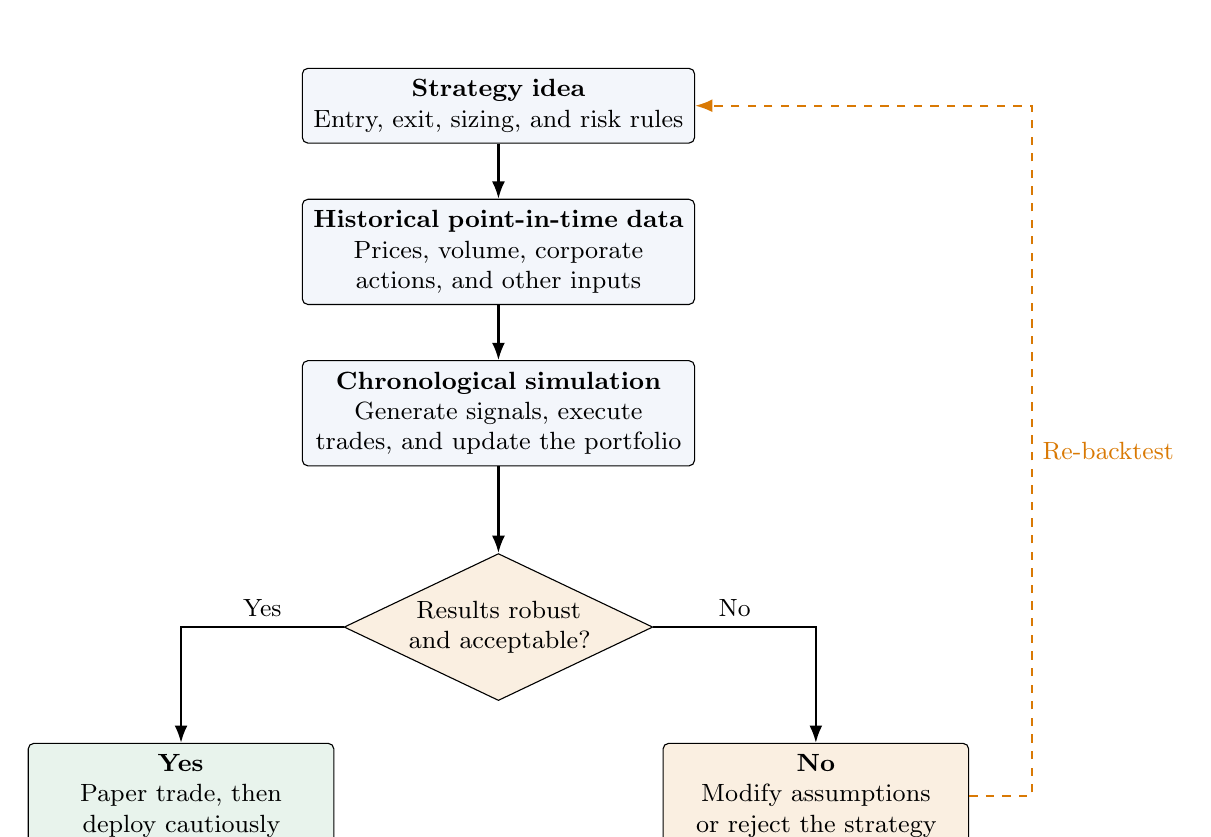
\begin{tikzpicture}[
    node distance=7mm and 13mm,
    every node/.style={font=\small},
    process/.style={diagramBox,text width=4.7cm,minimum height=9mm},
    outcome/.style={diagramBox,text width=3.6cm,minimum height=9mm}
]
\node[process] (idea) {\textbf{Strategy idea}\\Entry, exit, sizing, and risk rules};
\node[process,below=of idea] (data) {\textbf{Historical point-in-time data}\\Prices, volume, corporate actions, and other inputs};
\node[process,below=of data] (simulation) {\textbf{Chronological simulation}\\Generate signals, execute trades, and update the portfolio};
\node[diagramDecision,below=11mm of simulation,text width=2.3cm] (decision) {Results robust and acceptable?};
\node[outcome,below left=10mm and 11mm of decision,fill=diagramGreen!10] (positive)
{\textbf{Yes}\\Paper trade, then deploy cautiously};
\node[outcome,below right=10mm and 11mm of decision,fill=diagramOrange!12] (negative)
{\textbf{No}\\Modify assumptions or reject the strategy};

\draw[diagramArrow] (idea) -- (data);
\draw[diagramArrow] (data) -- (simulation);
\draw[diagramArrow] (simulation) -- (decision);
\draw[diagramArrow] (decision) -| node[pos=0.25,above]{Yes} (positive);
\draw[diagramArrow] (decision) -| node[pos=0.25,above]{No} (negative);
\draw[diagramArrow,diagramOrange,dashed]
  (negative.east) -- ++(8mm,0) |- node[pos=0.25,right]{Re-backtest} (idea.east);
\end{tikzpicture}
\caption{The basic backtesting and refinement cycle.}
\label{fig:backtesting-principle}
\end{figure}

\subsection{Requirements of a Good Backtest}

\begin{enumerate}
    \item \textbf{Quality historical data:} clean, complete, correctly
    adjusted, and free from survivorship bias.
    \item \textbf{Realistic simulation:} transaction costs, bid--ask
    spreads, slippage, latency, liquidity, and market impact are represented.
    \item \textbf{Appropriate time horizon:} the test covers several market
    regimes, including rising, falling, volatile, and sideways markets.
    \item \textbf{Rigorous evaluation:} several return and risk measures are
    considered rather than raw profit alone.
\end{enumerate}

\begin{quote}
\colorbox{diagramOrange!12}{%
\parbox{\dimexpr\linewidth-2\fboxsep\relax}{%
\textbf{Warning: overfitting.} A strategy that looks exceptional on the data
used to design it may merely have been tuned to historical noise. Reserve
unseen data for out-of-sample testing and use walk-forward validation before
drawing conclusions.}}
\end{quote}


\section{Performance Metrics for Backtesting a Trading Strategy}

\subsection{Overview}

Performance metrics permit objective comparisons among strategies.
\textbf{No single metric gives a complete assessment}; returns, risk, and
risk-adjusted performance should be examined together.

\begin{figure}[H]
\centering
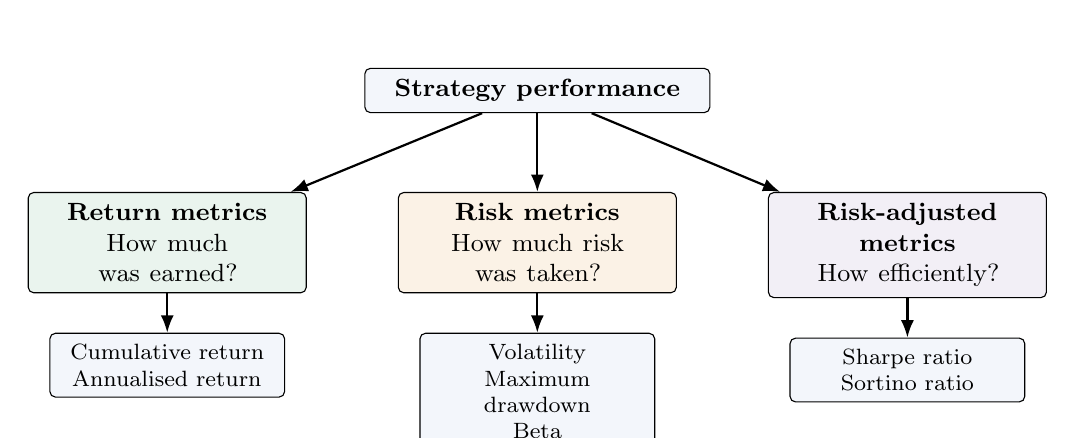
\begin{tikzpicture}[
    node distance=9mm and 6mm,
    category/.style={diagramBox,text width=3.25cm,minimum height=10mm,font=\small\bfseries},
    metric/.style={diagramBox,text width=2.7cm,minimum height=8mm,font=\footnotesize}
]
\node[diagramBox,text width=4.1cm,font=\small\bfseries] (root) {Strategy performance};

\node[category,below=10mm of root,xshift=-4.7cm,fill=diagramGreen!9] (ret)
{Return metrics\\{\normalfont How much was earned?}};
\node[category,below=10mm of root,fill=diagramOrange!10] (risk)
{Risk metrics\\{\normalfont How much risk was taken?}};
\node[category,below=10mm of root,xshift=4.7cm,fill=diagramPurple!9] (adj)
{Risk-adjusted metrics\\{\normalfont How efficiently?}};

\node[metric,below=5mm of ret] (cr) {Cumulative return\\Annualised return};
\node[metric,below=5mm of risk] (rm) {Volatility\\Maximum drawdown\\Beta};
\node[metric,below=5mm of adj] (ra) {Sharpe ratio\\Sortino ratio};

\draw[diagramArrow] (root) -- (ret);
\draw[diagramArrow] (root) -- (risk);
\draw[diagramArrow] (root) -- (adj);
\draw[diagramArrow] (ret) -- (cr);
\draw[diagramArrow] (risk) -- (rm);
\draw[diagramArrow] (adj) -- (ra);
\end{tikzpicture}
\caption{Three complementary views of strategy performance.}
\label{fig:performance-metric-groups}
\end{figure}

\subsection{Cumulative Return (Absolute Return)}

\textbf{Definition.} The total percentage gain or loss between the beginning
and end of the backtest, irrespective of its duration:
\[
\text{Cumulative return}
    = \frac{V_f-V_0}{V_0}\times 100\%,
\]
where \(V_0\) and \(V_f\) are the initial and final portfolio values.

\paragraph{Example.}
If a portfolio grows from Rs.\(1{,}00{,}000\) to
Rs.\(1{,}45{,}000\), then
\[
\frac{1{,}45{,}000-1{,}00{,}000}{1{,}00{,}000}\times100\%
   = \mathbf{45\%}.
\]

\textbf{Limitation.} Cumulative return ignores time. A \(45\%\) return over
ten years is not comparable with a \(45\%\) return earned in one year unless
both are annualised.

\subsection{Annualised Return}

\textbf{Definition.} The annualised return, or compound annual growth rate
(CAGR), is the constant yearly rate that produces the observed cumulative
return over the same period:
\[
\text{Annualised return}
 = \left(1+\text{cumulative return}\right)^{365/N}-1,
\]
where \(N\) is the number of calendar days in the backtest. If the duration
is expressed as \(T\) years, the exponent is \(1/T\).

\paragraph{Example.}
A cumulative return of \(45\%\) over \(547\) days gives
\[
(1.45)^{365/547}-1
  \approx (1.45)^{0.667}-1
  \approx \mathbf{28.1\%}.
\]

\begin{center}
\small
\begin{tabular}{|L{0.18\textwidth}|L{0.16\textwidth}|L{0.22\textwidth}|L{0.28\textwidth}|}
\hline
\textbf{Strategy} & \textbf{Duration} & \textbf{Cumulative return} &
\textbf{Annualised return} \\ \hline
A & 3 years & \(60\%\) & \((1.60)^{1/3}-1=16.96\%\) \\ \hline
B & 1.5 years & \(45\%\) & \((1.45)^{2/3}-1\approx28.1\%\) \\ \hline
\end{tabular}
\end{center}

Strategy B has the lower cumulative return but the higher annualised return
because it earned its gain in half the time.

\subsection{Annualised Volatility}

\textbf{Definition.} Volatility measures the dispersion of periodic returns.
For daily data it is commonly annualised as
\[
\sigma_{\mathrm{annual}}=\sigma_{\mathrm{daily}}\sqrt{252},
\]
where \(252\) is the conventional number of trading days in a year.

The square-root factor arises because independent return variances add over
time: annual variance is \(252\sigma_{\mathrm{daily}}^2\), so annual standard
deviation is \(\sqrt{252}\sigma_{\mathrm{daily}}\).

\paragraph{Example.}
For a daily standard deviation of \(1.3\%\),
\[
0.013\sqrt{252}=0.206\approx\mathbf{20.6\%}.
\]
Higher volatility means that realised returns are less stable. Thus, two
strategies with equal annualised returns can have very different risk
profiles.

\subsection{Sharpe Ratio}

\textbf{Definition.} The Sharpe ratio measures excess return per unit of
total volatility:
\[
\text{Sharpe ratio}=\frac{R_p-R_f}{\sigma_p},
\]
where \(R_p\) is the portfolio return, \(R_f\) is the risk-free return, and
\(\sigma_p\) is portfolio volatility. All three quantities must use the same
time scale.

\begin{center}
\small
\begin{tabular}{|L{0.20\textwidth}|L{0.65\textwidth}|}
\hline
\textbf{Sharpe ratio} & \textbf{Typical interpretation} \\ \hline
\(<0\) & The strategy earned less than the risk-free asset. \\ \hline
\(0\) to \(1\) & Positive but weak risk-adjusted performance. \\ \hline
\(1\) to \(2\) & Good risk-adjusted performance. \\ \hline
\(2\) to \(3\) & Very good risk-adjusted performance. \\ \hline
\(>3\) & Exceptional in a backtest; verify carefully for overfitting and omitted risks. \\ \hline
\end{tabular}
\end{center}

\paragraph{Worked example.}
For an annual strategy return of \(18\%\), an annual risk-free rate of
\(5\%\), and annualised volatility of \(12\%\),
\[
\text{Sharpe ratio}
 =\frac{18\%-5\%}{12\%}
 =\frac{13\%}{12\%}
 =\mathbf{1.08}.
\]

\paragraph{Limitations.}
\begin{itemize}
    \item Upside and downside volatility are penalised equally.
    \item The measure can understate tail risk when returns are skewed or
    heavy-tailed.
    \item Results are sensitive to the sampling frequency, annualisation
    convention, and chosen risk-free rate.
\end{itemize}

\subsection{Sortino Ratio}

\textbf{Definition.} The Sortino ratio replaces total volatility with
downside deviation, so only returns below a chosen target \(T\) are
penalised:
\[
\text{Sortino ratio}=\frac{R_p-R_f}{\sigma_{\mathrm{down}}},
\qquad
\sigma_{\mathrm{down}}
 =\sqrt{\frac{1}{n}\sum_{i=1}^{n}\min(0,R_i-T)^2}.
\]
The target may be zero, the risk-free rate, or another minimum acceptable
return.

\paragraph{Example.}
For periodic returns \(5\%,-3\%,8\%,-2\%,4\%\) and \(T=0\),
\[
\sigma_{\mathrm{down}}
 =\sqrt{\frac{(-3)^2+(-2)^2}{5}}
 =\sqrt{2.6}
 =1.61\%.
\]
If the annual return is \(12\%\), the risk-free rate is \(4\%\), and the
downside deviation has been expressed on the same annual scale, then
\[
\text{Sortino ratio}=\frac{12\%-4\%}{1.61\%}=4.97.
\]

The Sortino ratio is especially useful for asymmetric strategies, but a high
value should not be interpreted without examining rare tail losses.

\subsection{Beta}

\textbf{Definition.} Beta measures the sensitivity of a strategy to a market
benchmark:
\[
\beta=\frac{\operatorname{Cov}(R_p,R_m)}
            {\operatorname{Var}(R_m)},
\]
where \(R_p\) and \(R_m\) are portfolio and market returns.

\begin{center}
\small
\begin{tabular}{|L{0.15\textwidth}|L{0.40\textwidth}|L{0.28\textwidth}|}
\hline
\textbf{Beta} & \textbf{Meaning} & \textbf{Example} \\ \hline
\(\beta<0\) & Tends to move opposite to the market & Inverse or short strategies \\ \hline
\(\beta=0\) & No linear market exposure & Market-neutral strategy \\ \hline
\(0<\beta<1\) & Moves with the market, but less strongly & Defensive portfolio \\ \hline
\(\beta=1\) & Has the same market sensitivity as the benchmark & Index-tracking portfolio \\ \hline
\(\beta>1\) & Amplifies market movements & Leveraged or aggressive portfolio \\ \hline
\end{tabular}
\end{center}

\begin{figure}[H]
\centering
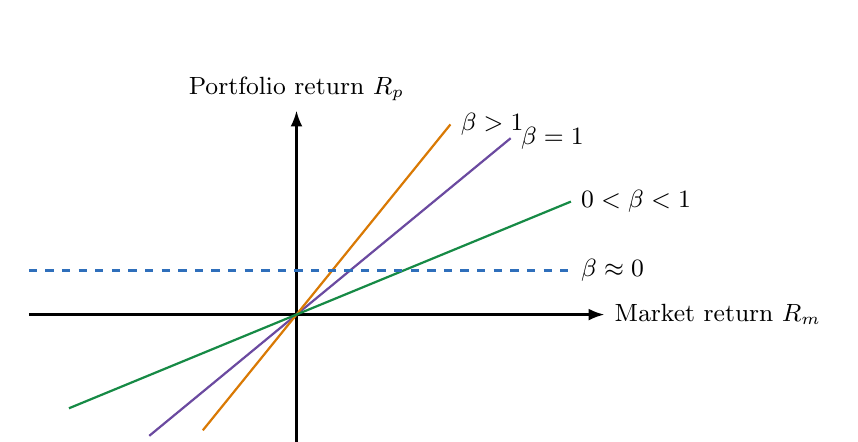
\begin{tikzpicture}[x=0.85cm,y=0.70cm,font=\small]
\draw[diagramAxis] (-4,0) -- (4.6,0) node[right]{Market return \(R_m\)};
\draw[diagramAxis] (0,-2.5) -- (0,3.7) node[above]{Portfolio return \(R_p\)};
\draw[diagramPurple,thick] (-2.2,-2.2) -- (3.2,3.2)
    node[right,black]{\(\beta=1\)};
\draw[diagramOrange,thick] (-1.4,-2.1) -- (2.3,3.45)
    node[right,black]{\(\beta>1\)};
\draw[diagramGreen,thick] (-3.4,-1.7) -- (4.1,2.05)
    node[right,black]{\(0<\beta<1\)};
\draw[diagramBlue,dashed,thick] (-4,0.8) -- (4.1,0.8)
    node[right,black]{\(\beta\approx0\)};
\end{tikzpicture}
\caption{Beta is the slope of the portfolio--market return relationship.}
\label{fig:beta-lines}
\end{figure}

A common single-factor decomposition is
\[
R_p=\alpha+\beta R_m+\varepsilon,
\]
where \(\alpha\) is benchmark-independent performance and \(\varepsilon\)
is unexplained variation. A high-return strategy with \(\beta=1.5\) may
mostly represent leveraged market exposure rather than a distinct trading
edge.

\subsection{Maximum Drawdown}

\textbf{Definition.} Maximum drawdown (MDD) is the largest peak-to-trough
decline in portfolio value before a new peak is reached. Its positive
magnitude is
\[
\text{MDD}
 =\max_t\left(\frac{P_t-V_t}{P_t}\right)\times100\%,
\qquad
P_t=\max_{s\leq t}V_s.
\]

\paragraph{Worked example.}
Consider the portfolio path
\[
\begin{aligned}
\text{Rs. }1{,}00{,}000
&\rightarrow \text{Rs. }1{,}50{,}000
\rightarrow \text{Rs. }90{,}000
\rightarrow \text{Rs. }1{,}20{,}000 \\
&\rightarrow \text{Rs. }70{,}000
\rightarrow \text{Rs. }1{,}60{,}000.
\end{aligned}
\]

\begin{figure}[H]
\centering
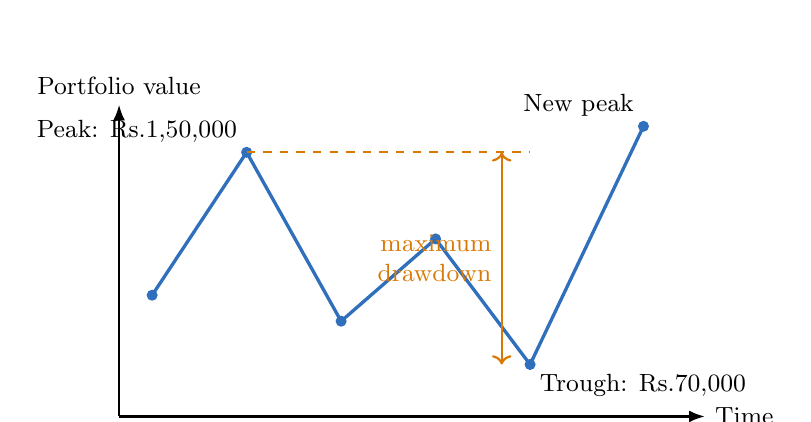
\begin{tikzpicture}[x=1.2cm,y=0.55cm,font=\small]
\draw[diagramAxis] (0,0) -- (6.2,0) node[right]{Time};
\draw[diagramAxis] (0,0) -- (0,7.2) node[above]{Portfolio value};
\draw[diagramBlue,very thick]
  (0.35,2.8) -- (1.35,6.1) -- (2.35,2.2) -- (3.35,4.1) --
  (4.35,1.2) -- (5.55,6.7);
\foreach \x/\y in {0.35/2.8,1.35/6.1,2.35/2.2,3.35/4.1,4.35/1.2,5.55/6.7}
  \fill[diagramBlue] (\x,\y) circle (2pt);
\draw[diagramOrange,dashed,thick] (1.35,6.1) -- (4.35,6.1);
\draw[diagramOrange,<->,thick] (4.05,1.2) -- (4.05,6.1)
  node[midway,left,align=right]{maximum\\drawdown};
\node[above left] at (1.35,6.1) {Peak: Rs.\(1{,}50{,}000\)};
\node[below right] at (4.35,1.2) {Trough: Rs.\(70{,}000\)};
\node[above left] at (5.55,6.7) {New peak};
\end{tikzpicture}
\caption{Maximum drawdown is measured from the preceding peak, not from the final value.}
\label{fig:maximum-drawdown}
\end{figure}

Thus,
\[
\text{MDD}
 =\frac{1{,}50{,}000-70{,}000}{1{,}50{,}000}\times100\%
 =\mathbf{53.33\%}.
\]
The interim recovery to Rs.\(1{,}20{,}000\) does not reset the peak because
it does not exceed Rs.\(1{,}50{,}000\).

A \(50\%\) loss requires a \(100\%\) subsequent gain merely to break even.
MDD therefore gives an intuitive capital-preservation and psychological
stress measure that volatility alone does not provide.

Two useful related measures are
\[
\text{Calmar ratio}
  =\frac{\text{annualised return}}{|\text{MDD}|},
\qquad
\text{Recovery factor}
  =\frac{\text{net profit}}{|\text{MDD}|}.
\]

\subsection{Summary of Performance Metrics}

\begin{center}
\footnotesize
\renewcommand{\arraystretch}{1.18}
\begin{tabular}{|L{0.15\textwidth}|L{0.23\textwidth}|L{0.21\textwidth}|L{0.15\textwidth}|}
\hline
\textbf{Metric} & \textbf{Formula} & \textbf{Measures} & \textbf{Preferred direction} \\ \hline
Cumulative return & \((V_f-V_0)/V_0\) & Total gain or loss & Higher \\ \hline
Annualised return & \((1+CR)^{365/N}-1\) & Compounded yearly growth & Higher \\ \hline
Annualised volatility & \(\sigma_d\sqrt{252}\) & Dispersion of returns & Lower, generally \\ \hline
Sharpe ratio & \((R_p-R_f)/\sigma_p\) & Excess return per unit of total risk & Higher \\ \hline
Sortino ratio & \((R_p-R_f)/\sigma_{\mathrm{down}}\) & Excess return per unit of downside risk & Higher \\ \hline
Beta & \(\operatorname{Cov}(R_p,R_m)/\operatorname{Var}(R_m)\) & Market sensitivity & Depends on objective \\ \hline
Maximum drawdown & \((P-T)/P\) & Worst peak-to-trough decline & Lower \\ \hline
\end{tabular}
\end{center}


\section{Slippage and Latency}

\subsection{What is Slippage?}

\textbf{Slippage} is the difference between the price observed when a signal
is generated and the price at which the order is actually filled:
\[
\text{Slippage magnitude}
 =\left|\text{execution price}-\text{signal price}\right|.
\]
For a buy order, execution above the signal price is adverse; for a sell
order, execution below the signal price is adverse.

\begin{quote}
\textbf{Example.} An algorithm generates a buy signal for HDFC Bank at
Rs.\(1{,}650.00\). The order is filled at Rs.\(1{,}651.25\), producing
adverse slippage of Rs.\(1.25\) per share.
\end{quote}

Slippage is a real transaction cost and can turn a small theoretical edge
into a loss.

\subsection{Why Slippage Occurs}

\begin{figure}[H]
\centering
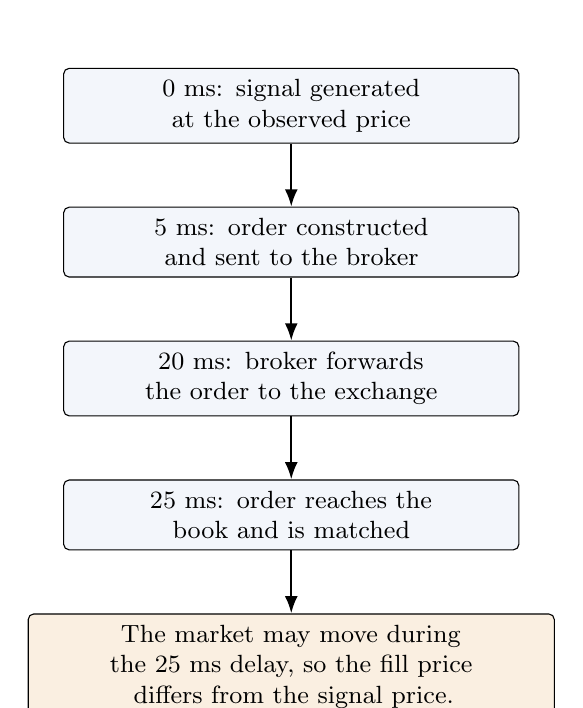
\begin{tikzpicture}[
  node distance=8mm,
  event/.style={diagramBox,text width=5.5cm,minimum height=8mm,font=\small}
]
\node[event] (s0) {\(0\) ms: signal generated at the observed price};
\node[event,below=of s0] (s1) {\(5\) ms: order constructed and sent to the broker};
\node[event,below=of s1] (s2) {\(20\) ms: broker forwards the order to the exchange};
\node[event,below=of s2] (s3) {\(25\) ms: order reaches the book and is matched};
\node[diagramBox,below=of s3,text width=6.4cm,fill=diagramOrange!12] (slip)
{The market may move during the \(25\) ms delay, so the fill price differs
from the signal price.};

\draw[diagramArrow] (s0) -- (s1);
\draw[diagramArrow] (s1) -- (s2);
\draw[diagramArrow] (s2) -- (s3);
\draw[diagramArrow] (s3) -- (slip);
\end{tikzpicture}
\caption{A simplified signal-to-execution latency chain.}
\label{fig:latency-chain}
\end{figure}

\subsection{Three Drivers of Slippage}

\subsubsection{Underlying Asset Volatility}

The farther a price can move per unit of time, the larger the range of
possible execution prices during a fixed delay.

\begin{figure}[H]
\centering
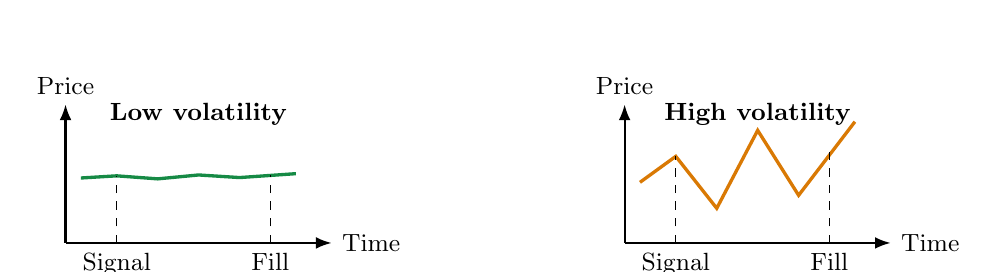
\begin{tikzpicture}[x=0.65cm,y=0.55cm,font=\small]
\begin{scope}
  \draw[diagramAxis] (0,0) -- (5.2,0) node[right]{Time};
  \draw[diagramAxis] (0,0) -- (0,3.2) node[above]{Price};
  \draw[diagramGreen,very thick]
    (0.3,1.5) -- (1.0,1.55) -- (1.8,1.48) -- (2.6,1.57) --
    (3.4,1.51) -- (4.5,1.60);
  \draw[dashed] (1.0,0) -- (1.0,1.55);
  \draw[dashed] (4.0,0) -- (4.0,1.56);
  \node[below] at (1.0,0) {Signal};
  \node[below] at (4.0,0) {Fill};
  \node[above] at (2.6,2.5) {\textbf{Low volatility}};
\end{scope}
\begin{scope}[xshift=7.1cm]
  \draw[diagramAxis] (0,0) -- (5.2,0) node[right]{Time};
  \draw[diagramAxis] (0,0) -- (0,3.2) node[above]{Price};
  \draw[diagramOrange,very thick]
    (0.3,1.4) -- (1.0,2.0) -- (1.8,0.8) -- (2.6,2.6) --
    (3.4,1.1) -- (4.5,2.8);
  \draw[dashed] (1.0,0) -- (1.0,2.0);
  \draw[dashed] (4.0,0) -- (4.0,2.3);
  \node[below] at (1.0,0) {Signal};
  \node[below] at (4.0,0) {Fill};
  \node[above] at (2.6,2.5) {\textbf{High volatility}};
\end{scope}
\end{tikzpicture}
\caption{The same execution delay creates more slippage uncertainty in a volatile asset.}
\label{fig:volatility-slippage}
\end{figure}

\begin{quote}
\textbf{Rule of thumb.} Higher short-horizon volatility generally implies
higher expected slippage, all else equal.
\end{quote}

\subsubsection{Latency}

\textbf{Latency} is the delay between signal generation and execution. It
includes:
\begin{itemize}
    \item \textbf{algorithmic latency}: time used to calculate the signal,
    perform checks, and construct the order; and
    \item \textbf{communication and execution latency}: time used to send
    the order through the broker, reach the exchange, queue, and obtain a fill.
\end{itemize}
Hence,
\[
\text{total latency}
 =\text{processing latency}
 +\text{communication and execution latency}.
\]

\begin{center}
\small
\begin{tabular}{|L{0.25\textwidth}|L{0.22\textwidth}|L{0.39\textwidth}|}
\hline
\textbf{Strategy type} & \textbf{Sensitivity} & \textbf{Reason} \\ \hline
High-frequency trading & Extremely high & Signals may decay within microseconds or milliseconds. \\ \hline
Intraday algorithms & Moderate to high & Opportunities often last seconds or minutes. \\ \hline
Swing or position trading & Usually lower & Signals are intended to persist for days or weeks. \\ \hline
\end{tabular}
\end{center}

This is why latency-sensitive firms may colocate servers near exchange
matching engines and use specialised networking or hardware.

\subsubsection{Strategy Type}

\begin{center}
\small
\begin{tabular}{|L{0.24\textwidth}|L{0.22\textwidth}|L{0.41\textwidth}|}
\hline
\textbf{Strategy} & \textbf{Typical impact} & \textbf{Reason} \\ \hline
Momentum & Often adverse & The strategy buys into rising prices or sells into falling prices. \\ \hline
Mean reversion & Can be less adverse, but is not guaranteed to be favourable &
The price may continue moving before reverting. \\ \hline
Market making & Two-sided and complex & Limit-order fills, queue position, spread capture, and adverse selection all matter. \\ \hline
\end{tabular}
\end{center}

\begin{figure}[H]
\centering
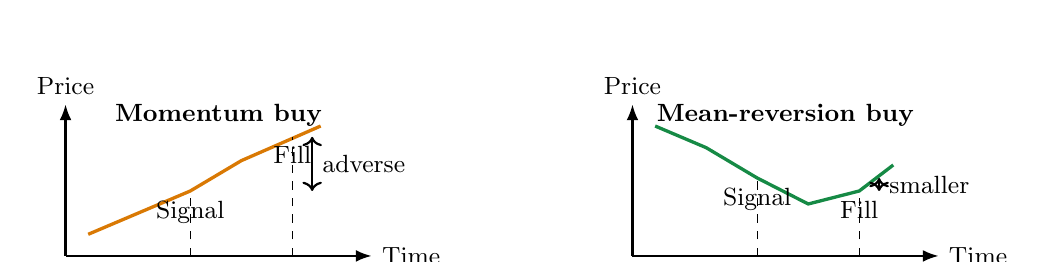
\begin{tikzpicture}[x=0.72cm,y=0.55cm,font=\small]
\begin{scope}
  \draw[diagramAxis] (0,0) -- (5.4,0) node[right]{Time};
  \draw[diagramAxis] (0,0) -- (0,3.5) node[above]{Price};
  \draw[diagramOrange,very thick] (0.4,0.5) -- (1.3,1.0) -- (2.2,1.5) --
    (3.1,2.2) -- (4.5,3.0);
  \draw[dashed] (2.2,0) -- (2.2,1.5) node[below]{Signal};
  \draw[dashed] (4.0,0) -- (4.0,2.75) node[below]{Fill};
  \draw[<->,thick] (4.35,1.5) -- (4.35,2.75)
    node[midway,right]{adverse};
  \node at (2.7,3.25) {\textbf{Momentum buy}};
\end{scope}
\begin{scope}[xshift=7.2cm]
  \draw[diagramAxis] (0,0) -- (5.4,0) node[right]{Time};
  \draw[diagramAxis] (0,0) -- (0,3.5) node[above]{Price};
  \draw[diagramGreen,very thick] (0.4,3.0) -- (1.3,2.5) -- (2.2,1.8) --
    (3.1,1.2) -- (4.0,1.5) -- (4.6,2.1);
  \draw[dashed] (2.2,0) -- (2.2,1.8) node[below]{Signal};
  \draw[dashed] (4.0,0) -- (4.0,1.5) node[below]{Fill};
  \draw[<->,thick] (4.35,1.5) -- (4.35,1.8)
    node[midway,right]{smaller};
  \node at (2.7,3.25) {\textbf{Mean-reversion buy}};
\end{scope}
\end{tikzpicture}
\caption{Illustrative, not guaranteed, slippage patterns for two strategy types.}
\label{fig:strategy-slippage}
\end{figure}


\section{Transaction Cost Models}

\subsection{Components of Transaction Costs}

Transaction costs include every cost caused by executing and maintaining a
trade. Omitting them can materially overstate backtested performance.
Important components include:
\begin{itemize}
    \item brokerage commissions;
    \item exchange fees, stamp duty, and taxes;
    \item the bid--ask spread;
    \item slippage and latency effects; and
    \item market impact, especially for orders large relative to available
    liquidity.
\end{itemize}

\subsection{Flat or Fixed Cost Model}

A fixed model assigns the same monetary cost to every trade:
\[
\text{total transaction cost}
 =C_{\mathrm{fixed}}N_{\mathrm{trades}}.
\]
For a fee of Rs.\(20\) per trade and \(500\) trades,
\[
\text{total cost}=\text{Rs. }20\times500=\text{Rs. }10{,}000.
\]

\paragraph{Advantages.}
It is simple, computationally inexpensive, and can represent genuinely
fixed per-order fees.

\paragraph{Disadvantages.}
It ignores trade size, liquidity, spread, volatility, slippage, and market
impact. It is therefore only a rough approximation for small and relatively
uniform orders.

\subsection{Linear Cost Model}

A linear model makes cost proportional to traded notional \(V\):
\[
\text{cost}=cV.
\]
For a \(0.1\%\) cost rate on a trade worth Rs.\(5{,}00{,}000\),
\[
\text{cost}=0.001\times\text{Rs. }5{,}00{,}000=\text{Rs. }500.
\]

A piecewise-linear specification may include a minimum charge, different
brokerage tiers, or different spread assumptions across size ranges. Linear
models are more realistic than fixed models for percentage fees, but they
still miss nonlinear market impact.

\subsection{Quadratic Cost Model}

A simple nonlinear approximation is
\[
\text{cost}=c_1V+c_2V^2,
\]
or, in a purely quadratic specification, \(\text{cost}=cV^2\). The
quadratic term approximates the increasing marginal cost of consuming more
levels of the order book.

For example, a purchase of \(100\) shares may be absorbed at the best ask,
whereas a purchase of \(10{,}000\) shares may consume several price levels.
The trader's own demand then raises the average execution price.

\begin{figure}[H]
\centering
\resizebox{0.98\textwidth}{!}{%
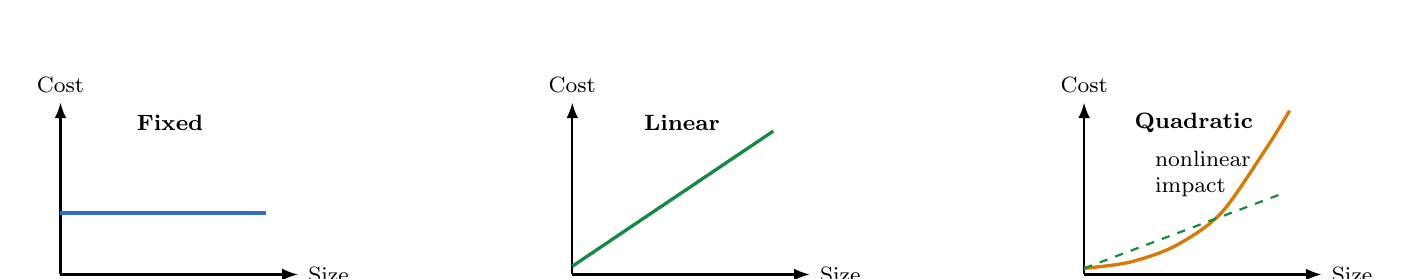
\begin{tikzpicture}[x=0.58cm,y=0.52cm,font=\footnotesize]
\begin{scope}
  \draw[diagramAxis] (0,0) -- (5.2,0) node[right]{Size};
  \draw[diagramAxis] (0,0) -- (0,4.2) node[above]{Cost};
  \draw[diagramBlue,very thick] (0,1.5) -- (4.5,1.5);
  \node at (2.4,3.7) {\textbf{Fixed}};
\end{scope}
\begin{scope}[xshift=6.5cm]
  \draw[diagramAxis] (0,0) -- (5.2,0) node[right]{Size};
  \draw[diagramAxis] (0,0) -- (0,4.2) node[above]{Cost};
  \draw[diagramGreen,very thick] (0,0.2) -- (4.4,3.5);
  \node at (2.4,3.7) {\textbf{Linear}};
\end{scope}
\begin{scope}[xshift=13cm]
  \draw[diagramAxis] (0,0) -- (5.2,0) node[right]{Size};
  \draw[diagramAxis] (0,0) -- (0,4.2) node[above]{Cost};
  \draw[diagramOrange,very thick]
    plot[smooth] coordinates {(0,0.15) (1,0.3) (2,0.7) (3,1.5) (4,3.1) (4.5,4.0)};
  \draw[diagramGreen,dashed,thick] (0,0.15) -- (4.4,2.0);
  \node at (2.4,3.7) {\textbf{Quadratic}};
  \node[align=left] at (2.6,2.45) {nonlinear\\impact};
\end{scope}
\end{tikzpicture}%
}
\caption{Fixed, linear, and quadratic transaction-cost approximations.}
\label{fig:transaction-cost-models}
\end{figure}

\paragraph{Advantages.}
A calibrated nonlinear model can represent market impact more realistically
when order size is material relative to liquidity.

\paragraph{Disadvantages.}
The coefficients must be estimated for each asset, venue, order type, and
market regime. A quadratic form is still an approximation; using it without
calibration does not guarantee accuracy.

\subsection{Using Historical Execution Costs}

A more data-driven cost model can be constructed as follows:
\begin{enumerate}
    \item collect fill prices, decision prices, order sizes, timestamps, and
    contemporaneous market conditions from executed orders;
    \item estimate slippage as a function of order size, volatility,
    liquidity, spread, participation rate, and latency; and
    \item apply the fitted model to simulated orders in the backtester.
\end{enumerate}

\begin{figure}[H]
\centering
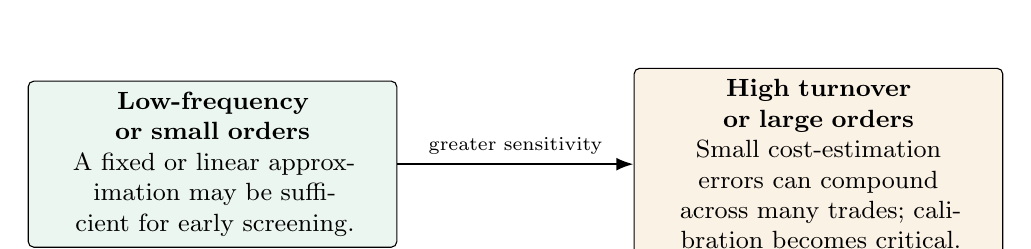
\begin{tikzpicture}[node distance=9mm and 30mm,font=\small]
\node[diagramBox,text width=4.4cm,fill=diagramGreen!8] (simple)
{\textbf{Low-frequency or small orders}\\A fixed or linear approximation
may be sufficient for early screening.};
\node[diagramBox,right=of simple,text width=4.4cm,fill=diagramOrange!10] (complex)
{\textbf{High turnover or large orders}\\Small cost-estimation errors can
compound across many trades; calibration becomes critical.};
\draw[diagramArrow] (simple) -- node[above,font=\scriptsize]{greater sensitivity} (complex);
\end{tikzpicture}
\caption{The required cost-model detail grows with turnover and market impact.}
\label{fig:cost-model-detail}
\end{figure}

For a high-turnover strategy, even a few basis points of omitted cost per
trade can consume the entire forecast edge.


\section{Backtesting Framework}

\subsection{Complete Workflow}

A rigorous backtest follows a staged process.

\begin{figure}[H]
\centering
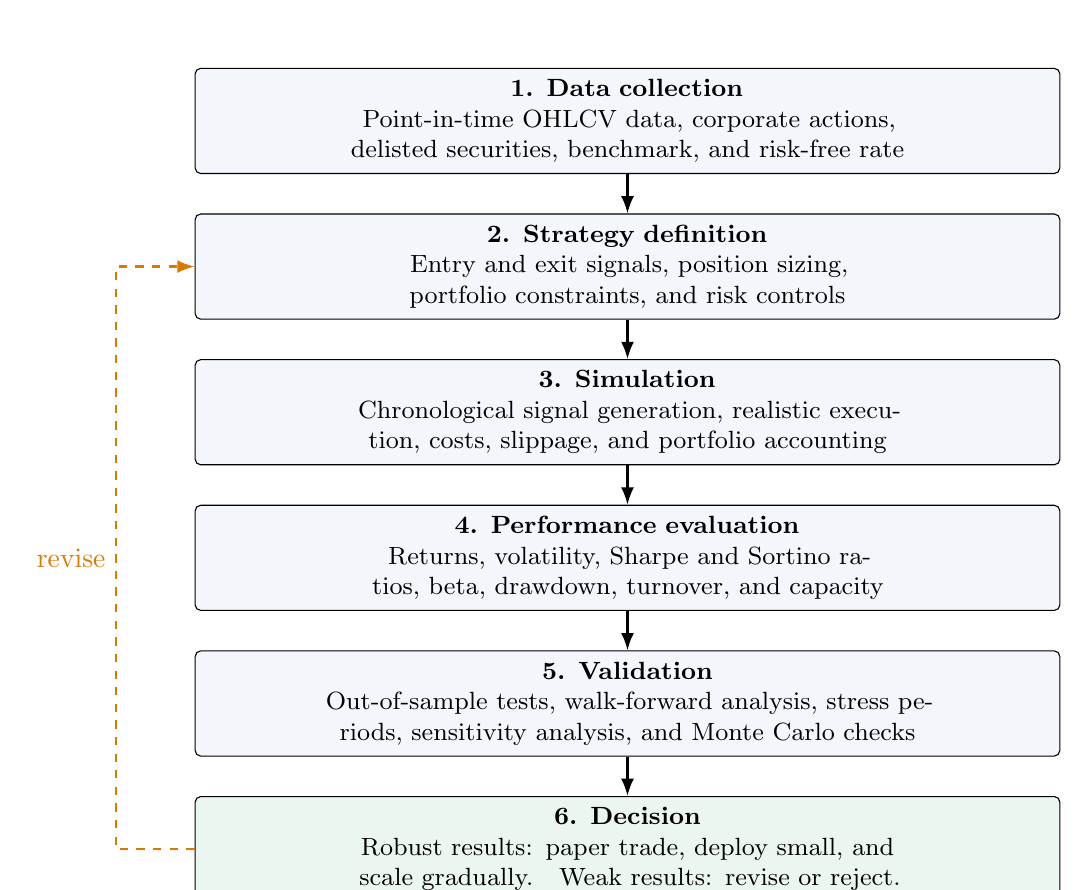
\begin{tikzpicture}[
  node distance=5mm,
  stage/.style={diagramBox,text width=10.7cm,minimum height=10mm,font=\small}
]
\node[stage] (data) {\textbf{1. Data collection}\\
Point-in-time OHLCV data, corporate actions, delisted securities, benchmark,
and risk-free rate};
\node[stage,below=of data] (rules) {\textbf{2. Strategy definition}\\
Entry and exit signals, position sizing, portfolio constraints, and risk controls};
\node[stage,below=of rules] (sim) {\textbf{3. Simulation}\\
Chronological signal generation, realistic execution, costs, slippage, and
portfolio accounting};
\node[stage,below=of sim] (eval) {\textbf{4. Performance evaluation}\\
Returns, volatility, Sharpe and Sortino ratios, beta, drawdown, turnover, and capacity};
\node[stage,below=of eval] (valid) {\textbf{5. Validation}\\
Out-of-sample tests, walk-forward analysis, stress periods, sensitivity
analysis, and Monte Carlo checks};
\node[stage,below=of valid,fill=diagramGreen!8] (decision) {\textbf{6. Decision}\\
Robust results: paper trade, deploy small, and scale gradually.\quad
Weak results: revise or reject.};

\draw[diagramArrow] (data) -- (rules);
\draw[diagramArrow] (rules) -- (sim);
\draw[diagramArrow] (sim) -- (eval);
\draw[diagramArrow] (eval) -- (valid);
\draw[diagramArrow] (valid) -- (decision);
\draw[diagramArrow,diagramOrange,dashed]
  (decision.west) -- ++(-10mm,0) |- node[pos=0.25,left]{revise} (rules.west);
\end{tikzpicture}
\caption{A complete backtesting and validation workflow.}
\label{fig:complete-backtesting-workflow}
\end{figure}

\subsection{Common Backtesting Pitfalls}

\subsubsection{Look-Ahead Bias}

Look-ahead bias occurs when the strategy uses information that was not
available at the simulated decision time. For example, today's closing price
cannot generate a trade executed earlier during today's session.

\textbf{Mitigation:} enforce strict timestamp ordering and delay execution
until after every required input would genuinely have been observable.

\subsubsection{Survivorship Bias}

Survivorship bias occurs when a historical universe contains only securities
that still exist today. Failed, delisted, or removed securities are omitted,
which can make past results look artificially strong.

\textbf{Mitigation:} use point-in-time index constituents and include all
securities that were investable on each historical date.

\subsubsection{Overfitting or Curve Fitting}

Overfitting occurs when parameters are tuned so aggressively that the
strategy captures noise specific to the development sample.

\textbf{Mitigation:} use a small number of economically justified
parameters, reserve out-of-sample data, perform walk-forward validation, and
test parameter sensitivity.

\subsubsection{Ignoring Transaction Costs}

Ignoring commissions, taxes, spreads, slippage, and market impact can turn an
unprofitable strategy into an apparently profitable one. For example, a
\(0.1\%\) round-trip cost repeated \(1{,}000\) times equals \(100\%\) of the
repeatedly traded notional, although its exact effect on portfolio return
depends on position size and turnover.

\textbf{Mitigation:} calibrate costs to the asset, venue, order type,
liquidity, trade size, and strategy frequency.

\subsubsection{Latency Blindness}

Latency blindness assumes an instantaneous fill at the signal price. In
practice, both the market and the available queue can change before an order
arrives.

\textbf{Mitigation:} delay fills realistically and model order type, queue
position, partial fills, and slippage at the relevant time scale.

\section{Libraries}

\subsection{Algorithmic Trading Libraries}

\begin{quote}
\textbf{Note on sources:} These notes are compiled from the official documentation and tutorials for each library (linked below), since these are the canonical, most reliable, and most current references. I was not able to transcribe the linked YouTube playlists directly (no video/audio access), but the concepts, functions, and worked examples they'd typically cover for these libraries are the same ones documented in the official tutorials, which are used here as the primary source. If you want specific clarifications that came from the videos and aren't reflected here, let me know what topic/timestamp and I can look into it further.

\end{quote}

\textbf{Sources used:}

\begin{itemize}
\item 
Pyfolio: \url{https://quantopian.github.io/pyfolio/} (Overview + all 6 tutorial notebooks)

\item 
Zipline (maintained fork \emph{zipline-reloaded}): \url{https://zipline.ml4trading.io/} (Tutorial + full API reference)

\item 
Zipline-trader (Alpaca-focused live-trading fork): \url{https://zipline-trader.readthedocs.io/en/latest/beginner-tutorial.html}

\item 
Backtesting.py: \url{https://kernc.github.io/backtesting.py/doc/backtesting/} (API docs, \texttt{backtesting.backtesting}, \texttt{backtesting.lib}) + Quick Start User Guide

\end{itemize}

\medskip
\hrule
\medskip
\subsubsection{Quick Orientation: Which Library Does What?}

\begin{longtable}{@{}L{0.22\textwidth}L{0.22\textwidth}L{0.22\textwidth}L{0.22\textwidth}@{}}
\toprule
\textbf{Library} & \textbf{Role} & \textbf{Scope} & \textbf{Best for} \\
\midrule
\textbf{Zipline} & Event-driven \textbf{backtesting simulator} (runs a strategy bar-by-bar) & Multi-asset, portfolio-level & Writing and \emph{simulating} a trading algorithm against historical data, including realistic order execution, slippage, commissions \\
\textbf{Pyfolio} & \textbf{Performance \& risk analytics} (post-hoc analysis) & Works on the \emph{output} (returns/positions/transactions) of a backtest (e.g. from Zipline) or even a single asset's returns & Generating professional "tear sheets" — the statistics and plots used to \emph{evaluate} a strategy after it has been run \\
\textbf{Backtesting.py} & Lightweight, single-asset \textbf{backtesting + optimization} framework & One tradeable asset at a time; not built for multi-asset portfolio rebalancing & Quickly prototyping, backtesting, and optimizing indicator/signal-based strategies with an intuitive, minimal API and interactive plots \\
\bottomrule
\end{longtable}

In short: you might \textbf{write and run} a strategy in \textbf{Zipline}, then \textbf{analyze its performance} with \textbf{Pyfolio} — or, for simpler single-asset strategy iteration, use \textbf{Backtesting.py} end-to-end (it has its own built-in stats and plotting, so it doesn't need Pyfolio).

\medskip
\hrule
\medskip
\subsection{Pyfolio}
\subsubsection{What It Is}

Pyfolio is a Python library for \textbf{performance and risk analysis of financial portfolios}, originally developed by Quantopian Inc. It integrates well with \textbf{Zipline} (Zipline produces the returns/positions/transactions data that Pyfolio analyzes), but it can just as easily analyze the returns of a single asset compared to a benchmark, or returns from any other source.

\textbf{Installation:}

\begin{python}
pip install pyfolio
\end{python}

(Bayesian tear sheets additionally require \texttt{pip install theano} and \texttt{pip install pymc3}.)
\subsubsection{The Core Concept: Tear Sheets}

At the heart of Pyfolio is the \textbf{tear sheet} — a collection of individual plots and statistics tables that together give a comprehensive picture of a strategy's performance. Rather than compute metrics one by one, you call one function and get a full battery of analysis at once.

The main tear-sheet-generating functions are:

\begin{longtable}{@{}L{0.46\textwidth}L{0.46\textwidth}@{}}
\toprule
\textbf{Function} & \textbf{Purpose} \\
\midrule
\texttt{pf.create\_returns\_tear\_sheet(returns, ...)} & Core statistics + plots based on a returns series alone (works even for a single stock) \\
\texttt{pf.create\_full\_tear\_sheet(returns, positions=None, transactions=None, ...)} & The "everything" tear sheet: returns stats + positions + transactions + (optionally) round trips + slippage sweeps \\
\texttt{pf.create\_position\_tear\_sheet(returns, positions, sector\_mappings=None)} & Analysis of holdings over time (top positions, sector allocation) \\
\texttt{pf.create\_round\_trip\_tear\_sheet(returns, positions, transactions, sector\_mappings=None)} & Analysis of individual "round trip" trades (win rate, profit factor, holding durations, etc.) \\
\bottomrule
\end{longtable}
\subsubsection{Required Input Data}

Pyfolio tear sheets are built from up to three pandas objects:

\begin{itemize}
\item 
\textbf{\texttt{returns}} — a \texttt{pd.Series} of daily percentage returns, datetime-indexed.

\item 
\textbf{\texttt{positions}} — a \texttt{pd.DataFrame} of daily dollar values held per symbol (plus a \texttt{'cash'} column), datetime-indexed.

\item 
\textbf{\texttt{transactions}} — a \texttt{pd.DataFrame} of individual trades executed (datetime-indexed), used for transaction-cost/slippage and round-trip analysis.

\end{itemize}

\paragraph{Getting a Single Stock's Returns}

\begin{python}
import pyfolio as pf
stock_rets = pf.utils.get_symbol_rets('FB')
pf.create_returns_tear_sheet(stock_rets, live_start_date='2015-12-1')
\end{python}

\texttt{live\_start\_date} splits the analysis into \textbf{in-sample} (before that date) and \textbf{out-of-sample} (after) — useful for checking whether a strategy's live performance matches its backtested performance.

\paragraph{Getting Data From a Zipline Backtest}

If you ran a strategy in Zipline and saved the results (\texttt{results.pickle}), Pyfolio can extract the three required objects directly:

\begin{python}
import pandas as pd
import pyfolio as pf

results = pd.read_pickle('results.pickle')
returns, positions, transactions = pf.utils.extract_rets_pos_txn_from_zipline(results)
\end{python}
\subsubsection{The Statistics Table (What Each Metric Means)}

Every \texttt{create\_*\_tear\_sheet} call prints a summary table like this (columns split into \textbf{All / In-sample / Out-of-sample} if \texttt{live\_start\_date} is given):

\begin{longtable}{@{}L{0.46\textwidth}L{0.46\textwidth}@{}}
\toprule
\textbf{Metric} & \textbf{Meaning} \\
\midrule
\textbf{Annual return} & Compounded annualized return \\
\textbf{Cumulative returns} & Total return over the whole period \\
\textbf{Annual volatility} & Annualized standard deviation of daily returns \\
\textbf{Sharpe ratio} & Risk-adjusted return: excess return per unit of total volatility \\
\textbf{Calmar ratio} & Annual return divided by max drawdown — rewards strategies with shallow drawdowns \\
\textbf{Stability} & R² of a linear fit to the log cumulative returns curve — how smooth/consistent the equity growth is \\
\textbf{Max drawdown} & Largest peak-to-trough decline in cumulative returns \\
\textbf{Omega ratio} & Probability-weighted ratio of gains vs. losses relative to a threshold \\
\textbf{Sortino ratio} & Like Sharpe, but only penalizes \emph{downside} volatility (not upside swings) \\
\textbf{Skew} & Asymmetry of the returns distribution (positive skew = more extreme gains than losses) \\
\textbf{Kurtosis} & "Fat-tailedness" of the returns distribution (high kurtosis = more extreme outlier days) \\
\textbf{Tail ratio} & Ratio of the size of the right tail (gains) to the left tail (losses), e.g. at the 95th vs. 5th percentile \\
\textbf{Daily value at risk} & Estimated daily loss threshold not expected to be exceeded except in the worst X\% of cases \\
\textbf{Gross leverage} & Total absolute exposure (long + short) relative to portfolio value \\
\textbf{Daily turnover} & How much of the portfolio is traded each day, as a fraction of portfolio value \\
\textbf{Alpha} & Return not explained by the benchmark (skill/edge) \\
\textbf{Beta} & Sensitivity of the strategy's returns to the benchmark's returns \\
\bottomrule
\end{longtable}

Below the summary table, tear sheets also show a \textbf{"Worst drawdown periods"} table listing each major drawdown's net decline (\%), peak date, valley date, recovery date, and duration (in days) — this makes it easy to see not just \emph{how deep} losses got but \emph{how long} the strategy stayed underwater.
\subsubsection{Plots Generated}

Depending on which tear sheet function is called, Pyfolio can generate:

\begin{itemize}
\item 
Cumulative returns plot (linear and log scale), vs. benchmark

\item 
Returns plot (per-period)

\item 
Rolling 6-month volatility

\item 
Rolling 6-month Sharpe ratio

\item 
Top 5 drawdown periods (highlighted on the cumulative returns curve)

\item 
Drawdown "underwater" plot (depth of drawdown over time)

\item 
Monthly returns heatmap (\%) and annual returns bar chart

\item 
Distribution of monthly returns (histogram)

\item 
Return quantiles box plot

\item 
Stress event table (mean/min/max returns during historical stress periods like the 2008 Lehman crisis, Aug '07, Mar '08, Sept '08, the 2009 recovery, etc.) — lets you see how the strategy would have behaved during known crisis windows

\item 
Top 10 long/short positions of all time, and all positions ever held (with sector breakdown, if \texttt{sector\_mappings} is supplied)

\end{itemize}
\subsubsection{Worked Example: Full Zipline Algorithm → Pyfolio Tear Sheet}

This is the canonical workflow: run a Zipline algorithm, save its output, then feed that output into Pyfolio.

\begin{python}
import pyfolio as pf
import zipline
%load_ext zipline
!zipline ingest   # download/prepare pricing data bundle first
\end{python}

\begin{python}
%%zipline --start 2004-1-1 --end 2010-1-1 -o results.pickle

# An "On-Line Portfolio Moving Average Reversion" (OLMAR) strategy
import numpy as np
from zipline.finance import commission, slippage

STOCKS = ['AMD', 'CERN', 'COST', 'DELL', 'GPS', 'INTC', 'MMM']

def initialize(algo, eps=1, window_length=5):
    algo.stocks = STOCKS
    algo.sids = [algo.symbol(s) for s in algo.stocks]
    algo.m = len(algo.stocks)
    algo.b_t = np.ones(algo.m) / algo.m   # start with an equal-weighted portfolio
    algo.eps = eps                         # reversion sensitivity parameter
    algo.window_length = window_length
    algo.set_commission(commission.PerShare(cost=0))
    algo.set_slippage(slippage.FixedSlippage(spread=0))

def handle_data(algo, data):
    # Compute each asset's price relative to its recent moving average
    mavgs = data.history(algo.sids, 'price', algo.window_length, '1d').mean()
    x_tilde = np.array([mavgs[sid] / data.current(sid, "price") for sid in algo.sids])
    # ... mean-reversion portfolio update logic (project onto the simplex
    # of valid portfolio weights) ...
    rebalance_portfolio(algo, data, new_weights)

def rebalance_portfolio(algo, data, desired_port):
    for i, sid in enumerate(algo.sids):
        algo.order_target_percent(sid, desired_port[i])
\end{python}

Then extract the results and feed them straight to Pyfolio:

\begin{python}
import pandas as pd
results = pd.read_pickle('results.pickle')
returns, positions, transactions = pf.utils.extract_rets_pos_txn_from_zipline(results)

# One plot at a time...
pf.plot_drawdown_periods(returns, top=5).set_xlabel('Date')

# ...or the full tear sheet, including round-trip trade analysis
pf.create_full_tear_sheet(returns, positions=positions, transactions=transactions,
                          live_start_date='2009-10-22', round_trips=True)
\end{python}

If you'd rather not reveal which specific symbols your strategy traded (e.g. when sharing a tear sheet publicly), pass \texttt{hide\_positions=True}:

\begin{python}
pf.create_full_tear_sheet(returns, positions=positions, transactions=transactions,
                          live_start_date='2009-10-22', hide_positions=True)
\end{python}
\subsubsection{Sector Analysis}

To break down PnL and position exposure by \textbf{sector} instead of just by symbol, pass a \texttt{sector\_mappings} dictionary (symbol → sector name):

\begin{python}
sect_map = {'COST': 'Consumer Goods', 'INTC': 'Technology', 'CERN': 'Healthcare',
            'GPS': 'Technology', 'MMM': 'Construction', 'DELL': 'Technology', 'AMD': 'Technology'}

pf.create_position_tear_sheet(returns, positions, sector_mappings=sect_map)
# or, for round trips:
pf.create_round_trip_tear_sheet(returns, positions, transactions, sector_mappings=sect_map)
\end{python}

This adds a "Profitability (PnL / PnL total) per name" table aggregated at the \textbf{sector} level in addition to the per-symbol table, which is useful for spotting concentration risk (e.g. "is my strategy's profit really coming from one sector?").
\subsubsection{Round-Trip Trade Analysis}

A \textbf{round trip trade} begins when a new long or short position is opened, and ends when it is completely or partially closed. Round-trip analysis exists to answer: \emph{is this strategy repeatedly profitable, or did a few lucky trades carry the whole equity curve?}

\textbf{How it works under the hood:} Pyfolio reconstructs your full portfolio from the \texttt{transactions} you provide. When a new trade occurs, it checks whether shares of that symbol are already held from an earlier purchase; if so, it computes the PnL, return, and duration of that "round trip." At the very end of the data, any still-open positions are synthetically closed out (using the last available price) so that their PnL is captured too.

\begin{python}
pf.create_round_trip_tear_sheet(returns, positions, transactions, sector_mappings=sect_map)
\end{python}

This produces four groups of statistics, each broken down into \textbf{All trades / Short trades / Long trades}:

\begin{longtable}{@{}L{0.30\textwidth}L{0.30\textwidth}L{0.30\textwidth}@{}}
\toprule
\textbf{Stat group} & \textbf{Key fields} & \textbf{Meaning} \\
\midrule
\textbf{Summary stats} & Total \# round trips, Percent profitable, Winning/Losing/Even round trips & Basic win-rate bookkeeping \\
\textbf{PnL stats} & Total profit, Gross profit, Gross loss, Profit factor, Avg./Largest winning \& losing trade & Profit factor = gross profit / |gross loss|; a value > 1 means the strategy makes more from winners than it loses from losers \\
\textbf{Duration stats} & Avg./Median/Longest/Shortest duration & How long, on average, capital is tied up in a trade \\
\textbf{Return stats} & Avg./Median returns (all / winning / losing), largest winning/losing trade (\%) & Same PnL picture but expressed as \% return per round trip rather than \$ \\
\bottomrule
\end{longtable}

There's also a \textbf{per-symbol breakdown} of all the above (so you can see, e.g., that one ticker in your universe was actually a net drag on performance), and a \textbf{"Profitability per name"} bar chart.

\textbf{Under the hood, manually:}

\begin{python}
rts = pf.round_trips.extract_round_trips(
    transactions, portfolio_value=positions.sum(axis='columns') / (returns + 1))
pf.round_trips.print_round_trip_stats(rts)
\end{python}

\texttt{rts} is itself a DataFrame with one row per round trip: \texttt{close\_dt}, \texttt{long} (bool), \texttt{open\_dt}, \texttt{pnl}, \texttt{rt\_returns}, \texttt{symbol}, \texttt{duration}, \texttt{returns}.
\subsubsection{Slippage Sensitivity Analysis}

\textbf{Slippage} is the difference between the price you expected to trade at and the price you actually got — it eats into real-world returns in a way backtests often underestimate. Pyfolio's transactions tear sheet can generate \textbf{"slippage sweep"} plots showing how the strategy's equity curve would look under a range of additional per-dollar slippage assumptions.

\begin{python}
pf.create_full_tear_sheet(returns, positions, transactions, slippage=5)
\end{python}

Here, \texttt{slippage} is specified in \textbf{basis points} (1\% = 100 bps). Passing \texttt{slippage=5} applies 5 bps of \emph{additional} slippage on top of whatever is already baked into the returns you passed in, and shows the resulting performance for the main tear sheet plots.

\textbf{Important nuance:} the slippage sweep plots themselves always show a \emph{range} of slippage scenarios (e.g. 0, 1, 2, 5, 10 bps) for comparison — the \texttt{slippage=N} argument only affects the \emph{main} returns/plots elsewhere in the tear sheet, not the sweep itself. If your \texttt{returns} already reflect realistic slippage (e.g. from a proper Zipline backtest with a slippage model), pass \texttt{slippage=0} so you don't double-count, while still getting the sweep plot for comparison purposes.
\subsubsection{Bayesian Tear Sheet}

Pyfolio also offers a \textbf{Bayesian} analysis (requires PyMC3 + Theano) that models strategy returns probabilistically rather than with simple point-estimate statistics — e.g. giving credible intervals for the Sharpe ratio rather than a single number, and modeling the probability distribution of future drawdowns. This is more advanced/experimental and is best explored via the linked example notebook rather than summarized here, since it's essentially a from-scratch probabilistic model rather than a fixed formula.

\medskip
\hrule
\medskip
\subsection{Zipline}
\subsubsection{What It Is and Current Status}

Zipline is an \textbf{open-source, event-driven algorithmic trading simulator} written in Python, originally built by Quantopian as the engine behind their backtesting and live-trading platform. When Quantopian shut down in late 2020, its original documentation domain (\texttt{zipline.io}) expired.

\textbf{Important:} the documentation used here is for \textbf{\texttt{zipline-reloaded}}, the actively maintained community fork (maintained by Stefan Jansen, author of \emph{Machine Learning for Algorithmic Trading}) — this is the version you should actually install today, via:

\begin{python}
pip install zipline-reloaded
# or
conda install -c conda-forge zipline-reloaded
\end{python}

There is also a separate fork, \textbf{\texttt{zipline-trader}}, aimed specifically at connecting Zipline to the Alpaca brokerage for \textbf{live trading}, not just backtesting — its beginner tutorial content is functionally identical to the core Zipline tutorial (same \texttt{initialize}/\texttt{handle\_data} API), but it adds bundle ingestion via Alpaca, a YAML config file, and a "Going Live" mode.

Key stated benefits of Zipline:

\begin{itemize}
\item \textbf{Realistic}: models slippage, transaction costs, and order delays.

\item \textbf{Stream-based}: processes each time-bar event individually, which helps avoid look-ahead bias.

\item \textbf{Batteries included}: common transforms (e.g. moving averages) and risk stats (e.g. Sharpe) are available out of the box.

\item \textbf{PyData integration}: input/output are Pandas DataFrames.

\end{itemize}
\subsubsection{The Core Algorithm Structure}

Every Zipline algorithm is built around \textbf{two required functions}:

\begin{python}
def initialize(context):
    ...  # called once, before the backtest starts

def handle_data(context, data):
    ...  # called once per event (trading bar)
\end{python}

\begin{itemize}
\item 
\textbf{\texttt{initialize(context)}} runs once at the very start. \texttt{context} is a persistent namespace object — anything you store on it (\texttt{context.i = 0}, \texttt{context.asset = ...}) is available in every later call.

\item 
\textbf{\texttt{handle\_data(context, data)}} runs once per bar (once per day, for daily data; once per minute, for minute data). \texttt{data} is a \texttt{BarData} object giving you access to current and historical price/volume info for your universe.

\end{itemize}

Two additional optional functions:

\begin{itemize}
\item 
\textbf{\texttt{before\_trading\_start(context, data)}} — runs once per day, before the market opens (good place to run/refresh a Pipeline).

\item 
\textbf{\texttt{analyze(context, perf)}} — runs once, automatically, after the whole backtest finishes; \texttt{perf} is the full performance DataFrame, useful for custom plotting.

\end{itemize}

\paragraph{Minimal Example (\texttt{buyapple.py})}

\begin{python}
from zipline.api import order, record, symbol

def initialize(context):
    pass

def handle_data(context, data):
    order(symbol('AAPL'), 10)  # buy 10 shares of AAPL every bar
    record(AAPL=data.current(symbol('AAPL'), 'price'))
\end{python}

\begin{itemize}
\item 
\texttt{order()} takes an asset object and a signed integer amount — positive to buy/cover, negative to sell/short.

\item 
\texttt{record()} saves a named value on every bar; after the run finishes, these appear as columns in the performance DataFrame (letting you plot e.g. your own custom indicator alongside portfolio value).

\end{itemize}
\subsubsection{The \texttt{BarData} Object (\texttt{data})}

Passed into \texttt{handle\_data}/\texttt{before\_trading\_start}, this is your window into current and historical prices.

\paragraph{\texttt{data.current(assets, fields)}}

Returns the \emph{current} bar's value(s) for one or more assets/fields.

\begin{itemize}
\item 
Valid \texttt{fields}: \texttt{"price"}, \texttt{"open"}, \texttt{"high"}, \texttt{"low"}, \texttt{"close"}, \texttt{"volume"}, \texttt{"last\_traded"}.

\item 
\texttt{"price"} = last known close, forward-filled if no trade happened this bar, and split/dividend-adjusted.

\item 
\texttt{"open"/"high"/"low"/"close"} = NaN if there was no trade this bar.

\item 
\texttt{"volume"} = 0 if no trade this bar.

\item 
Return type depends on inputs: scalar (1 asset, 1 field) → \texttt{pd.Series} (1 asset+many fields, or many assets+1 field) → \texttt{pd.DataFrame} (many assets+many fields).

\end{itemize}

\paragraph{\texttt{data.history(assets, fields, bar\_count, frequency)}}

Returns a \textbf{trailing window} of historical data — this is how you get access to "yesterday's" or "last N days'" prices, adjusted for splits/dividends/mergers as of \emph{now} (so no look-ahead bias creeps in via unadjusted historical prices).

\begin{itemize}
\item 
\texttt{frequency}: \texttt{'1d'} for daily bars, \texttt{'1m'} for minute bars (needs minute-resolution data ingested).

\item 
\texttt{bar\_count}: how many historical bars to return.

\item 
Shape of the return value follows the same "scalar / Series / DataFrame" logic as \texttt{.current()}, with the extra wrinkle that multi-asset + multi-field requests return a \texttt{MultiIndex} DataFrame.

\end{itemize}

\paragraph{\texttt{data.can\_trade(assets)} / \texttt{data.is\_stale(assets)}}

\begin{itemize}
\item 
\texttt{can\_trade()}: True only if the asset is alive, its exchange is open right now, and there's a known last price for it — use this before ordering to avoid errors on delisted/inactive assets.

\item 
\texttt{is\_stale()}: True if the asset is alive but simply hasn't traded in the current bar (helps distinguish "no recent data" from "doesn't exist").

\end{itemize}
\subsubsection{Dual Moving Average Example (Using \texttt{history})}

This is the canonical "beyond the basics" tutorial example, and it introduces the idea of \textbf{precomputing indicators from a rolling history window}:

\begin{python}
from zipline.api import order_target, record, symbol

def initialize(context):
    context.i = 0
    context.asset = symbol('AAPL')

def handle_data(context, data):
    context.i += 1
    if context.i < 300:
        return  # skip until we have a full 300-bar window

    short_mavg = data.history(context.asset, 'price', bar_count=100, frequency="1d").mean()
    long_mavg  = data.history(context.asset, 'price', bar_count=300, frequency="1d").mean()

    if short_mavg > long_mavg:
        order_target(context.asset, 100)   # go/stay long 100 shares
    elif short_mavg < long_mavg:
        order_target(context.asset, 0)     # flatten the position

    record(AAPL=data.current(context.asset, 'price'),
           short_mavg=short_mavg, long_mavg=long_mavg)

def analyze(context, perf):
    import matplotlib.pyplot as plt
    fig = plt.figure()
    ax1 = fig.add_subplot(211); perf.portfolio_value.plot(ax=ax1)
    ax2 = fig.add_subplot(212); perf['AAPL'].plot(ax=ax2)
    perf[['short_mavg', 'long_mavg']].plot(ax=ax2)
    plt.show()
\end{python}

\textbf{Logic:} this is a classic momentum "golden cross / death cross" strategy — go long when the short-term average crosses above the long-term average (recent prices trending up relative to the longer trend), and exit when it crosses back below.

\textbf{A subtlety worth remembering:} \texttt{order\_target()} (like all the "target" order functions) does \textbf{not} account for orders you've already placed but which haven't filled yet. Calling \texttt{order\_target(asset, 10)} twice in a row (before either fills) results in \textbf{20 shares total}, not 10 — because Zipline doesn't yet know the first order will succeed when it processes the second.
\subsubsection{Running an Algorithm: Three Interfaces}

\paragraph{A. Command Line}

\begin{python}
zipline ingest -b quandl      # first: download/prepare a data bundle
zipline run -f my_algo.py --start 2016-1-1 --end 2018-1-1 -o results.pickle --no-benchmark
\end{python}

Key \texttt{zipline run} flags:

\begin{longtable}{@{}L{0.46\textwidth}L{0.46\textwidth}@{}}
\toprule
\textbf{Flag} & \textbf{Purpose} \\
\midrule
\texttt{-f/--algofile} & Path to your algorithm's \texttt{.py} file \\
\texttt{-b/--bundle} & Which ingested data bundle to use (default \texttt{quandl}) \\
\texttt{-s/--start}, \texttt{-e/--end} & Backtest date range \\
\texttt{--data-frequency} & \texttt{daily} (default) or \texttt{minute} \\
\texttt{--capital-base} & Starting cash (default 10,000,000) \\
\texttt{-o/--output} & Where to save the resulting performance DataFrame (pickle format) \\
\texttt{--benchmark-symbol} / \texttt{--benchmark-sid} / \texttt{--benchmark-file} & What to use as the benchmark for alpha/beta calculations \\
\texttt{--no-benchmark} & Skip a benchmark entirely (alpha/beta won't be computed) \\
\texttt{--trading-calendar} & Which market calendar to simulate against (default NYSE) \\
\bottomrule
\end{longtable}

Zipline first calls \texttt{initialize()}, then streams historical bars through \texttt{handle\_data()} day by day (or minute by minute). After \texttt{handle\_data()} returns each bar, Zipline looks at any orders placed and tries to fill them against that bar's volume — applying the configured commission and slippage models, so the true cost is more than just \texttt{price × shares}.

\paragraph{B. Jupyter Notebook Magic}

\begin{python}
%load_ext zipline
\end{python}

\begin{python}
%%zipline --start 2016-1-1 --end 2018-1-1 -o perf_variable
from zipline.api import symbol, order, record

def initialize(context):
    pass

def handle_data(context, data):
    order(symbol('AAPL'), 10)
    record(AAPL=data.current(symbol('AAPL'), 'price'))
\end{python}

Same CLI-style flags apply, but the algorithm lives inline in the notebook cell, and \texttt{-o name} creates a Python variable (rather than writing a file) holding the resulting DataFrame.

\paragraph{C. \texttt{run\_algorithm()} — for Running Like a Normal Script/IDE}

\begin{python}
from zipline import run_algorithm
import pandas as pd
import pandas_datareader.data as web

start = pd.Timestamp('2014'); end = pd.Timestamp('2018')
sp500 = web.DataReader('SP500', 'fred', start, end).SP500
benchmark_returns = sp500.pct_change()

result = run_algorithm(
    start=start.tz_localize('UTC'), end=end.tz_localize('UTC'),
    initialize=initialize, handle_data=handle_data,
    capital_base=100000, benchmark_returns=benchmark_returns,
    bundle='quandl', data_frequency='daily')
\end{python}

This is the most flexible option since it's just a Python function call — good for running inside an IDE, a script, or a testing/CI pipeline.
\subsubsection{The Performance DataFrame}

Whichever way you run it, Zipline returns/saves a \texttt{pd.DataFrame} with \textbf{one row per trading day (or minute)}. Key columns include:

\begin{longtable}{@{}L{0.46\textwidth}L{0.46\textwidth}@{}}
\toprule
\textbf{Column} & \textbf{Meaning} \\
\midrule
\texttt{portfolio\_value} & Total account value (cash + holdings) at that point \\
\texttt{returns} & Period return \\
\texttt{algorithm\_period\_return} / \texttt{benchmark\_period\_return} & Cumulative return so far, strategy vs. benchmark \\
\texttt{alpha}, \texttt{beta}, \texttt{sharpe}, \texttt{sortino} & Rolling risk/performance stats, computed automatically \\
\texttt{algo\_volatility}, \texttt{benchmark\_volatility} & Rolling annualized volatility \\
\texttt{max\_drawdown} & Running max drawdown to date \\
\texttt{positions} & List of currently held positions (dicts, with sid, amount, cost basis, last sale price, etc.) \\
\texttt{transactions} & List of any fills that happened this bar \\
\texttt{orders} & List of any orders created/updated this bar \\
\texttt{ending\_cash}, \texttt{ending\_value}, \texttt{ending\_exposure} & Cash and market value of holdings at end of bar \\
\texttt{longs\_count} / \texttt{shorts\_count}, \texttt{long\_value} / \texttt{short\_value} & Breakdown of long vs. short exposure \\
\texttt{gross\_leverage} / \texttt{net\_leverage} & Leverage measures \\
Any name you passed to \texttt{record()} & Your custom tracked values (e.g. \texttt{AAPL}, \texttt{short\_mavg}) \\
\bottomrule
\end{longtable}
\subsubsection{Placing Orders}

\begin{longtable}{@{}L{0.46\textwidth}L{0.46\textwidth}@{}}
\toprule
\textbf{Function} & \textbf{Semantics} \\
\midrule
\texttt{order(asset, amount, limit\_price=None, stop\_price=None, style=None)} & Order a \textbf{fixed number of shares} (+ = buy/cover, − = sell/short) \\
\texttt{order\_value(asset, value, ...)} & Order enough shares to transact a \textbf{fixed dollar value}. Equivalent to \texttt{order(asset, value / current\_price)} \\
\texttt{order\_percent(asset, percent, ...)} & Order enough shares to allocate a given \textbf{\% of current portfolio value} to the asset \\
\texttt{order\_target(asset, target, ...)} & Order the difference needed so the position reaches a \textbf{target share count} \\
\texttt{order\_target\_value(asset, target, ...)} & Same, but target is a \textbf{dollar value} (for Futures, this becomes target \emph{exposure}, since futures have no "value" per se) \\
\texttt{order\_target\_percent(asset, target, ...)} & Same, but target is a \textbf{\% of portfolio value} \\
\bottomrule
\end{longtable}

\textbf{Critical caveat repeated in the docs for all four "target" functions:} none of them account for your own still-open orders. Calling the same \texttt{order\_target*} twice before the first fills will double the effect, since each call only looks at your \emph{current filled} position, not your pending orders.

\paragraph{Execution Styles (how/when an order fills)}

\begin{itemize}
\item 
\textbf{\texttt{MarketOrder}} (default) — filled at the current/next available market price.

\item 
\textbf{\texttt{LimitOrder(limit\_price)}} — filled only at \texttt{limit\_price} or better.

\item 
\textbf{\texttt{StopOrder(stop\_price)}} — becomes a market order once price crosses \texttt{stop\_price} (in the direction that would normally hurt you, i.e. this is a protective/breakout trigger).

\item 
\textbf{\texttt{StopLimitOrder(limit\_price, stop\_price)}} — combination: becomes a \emph{limit} order once the stop price is triggered.

\end{itemize}

You can pass \texttt{limit\_price=} / \texttt{stop\_price=} directly to \texttt{order()} as shorthand instead of constructing a style object explicitly (but not both a \texttt{style=} and \texttt{limit\_price=}/\texttt{stop\_price=} at once).

\paragraph{Managing Orders}

\begin{itemize}
\item 
\texttt{get\_order(order\_id)} — look up a specific order.

\item 
\texttt{get\_open\_orders(asset=None)} — all open orders (dict of asset → list, or a list if \texttt{asset} given).

\item 
\texttt{cancel\_order(order\_param)} — cancel by ID or Order object.

\item 
\textbf{Cancel policies} — \texttt{set\_cancel\_policy(cancel\_policy)}, with built-ins \texttt{EODCancel()} (cancel all open orders at end of day; minute-frequency sims only) and \texttt{NeverCancel()} (default; orders are Good-Til-Canceled).

\end{itemize}
\subsubsection{Looking Up Assets}

\begin{itemize}
\item 
\texttt{symbol(symbol\_str, country\_code=None)} — look up a single Equity by ticker (as of the "symbol lookup date," since tickers can be reused by different companies over time).

\item 
\texttt{symbols(*args)} — look up several tickers at once, returns a list.

\item 
\texttt{future\_symbol(symbol)} — look up a Future contract by its symbol.

\item 
\texttt{sid(sid)} — look up any Asset by its permanent integer ID (doesn't change over time, unlike ticker symbols).

\item 
\texttt{set\_symbol\_lookup\_date(dt)} — change the reference date used to resolve ticker symbols to assets.

\end{itemize}
\subsubsection{Trading Controls (Safety Rails)}

These raise a \texttt{TradingControlException} if violated — designed to prevent a bug (or, on a live account, a fat-finger) from doing serious damage:

\begin{itemize}
\item 
\texttt{set\_do\_not\_order\_list(restricted\_list)} — assets that can never be ordered.

\item 
\texttt{set\_long\_only()} — disallow short positions entirely.

\item 
\texttt{set\_max\_leverage(max\_leverage)} — cap on account leverage.

\item 
\texttt{set\_max\_order\_count(max\_count)} — cap on number of orders per day.

\item 
\texttt{set\_max\_order\_size(asset=None, max\_shares=None, max\_notional=None)} — cap the size of any single order.

\item 
\texttt{set\_max\_position\_size(asset=None, max\_shares=None, max\_notional=None)} — cap the size of any resulting position (note: splits/dividends or price moves can still push you slightly over after the fact).

\end{itemize}
\subsubsection{Commission and Slippage Models}

These model the two main sources of "backtest looks better than reality" error.

\textbf{Commission} (\texttt{set\_commission(us\_equities=..., us\_futures=...)}), can only be set inside \texttt{initialize()}:

\begin{longtable}{@{}L{0.46\textwidth}L{0.46\textwidth}@{}}
\toprule
\textbf{Model} & \textbf{Formula} \\
\midrule
\texttt{commission.PerShare(cost=0.001, min\_trade\_cost=0.0)} & Flat \$ per share traded, with an optional minimum per trade. \textbf{This is Zipline's default for equities.} \\
\texttt{commission.PerTrade(cost=0.0)} & Flat \$ per trade regardless of size (multi-fill orders charge the full amount on the first fill) \\
\texttt{commission.PerDollar(cost=0.0015)} & \$ cost proportional to dollar value transacted (default 0.15\% of value) \\
\bottomrule
\end{longtable}

You can also subclass \texttt{CommissionModel} and implement \texttt{calculate(order, transaction)} for custom logic.

\textbf{Slippage} (\texttt{set\_slippage(us\_equities=..., us\_futures=...)}):

\begin{longtable}{@{}L{0.46\textwidth}L{0.46\textwidth}@{}}
\toprule
\textbf{Model} & \textbf{Formula / Behavior} \\
\midrule
\texttt{slippage.FixedSlippage(spread=0.0)} & Buys fill at \texttt{close + spread/2}; sells fill at \texttt{close - spread/2}. No volume/liquidity limit — will always fill in full as soon as \emph{any} trading occurs, even if your order is bigger than the historical volume (unrealistic for large orders, but simple). \\
\texttt{slippage.VolumeShareSlippage(volume\_limit=0.025, price\_impact=0.1)} & Models slippage as a function of how much of the bar's volume your order represents. Buys fill at \texttt{price * (1 + price\_impact * volume\_share**2)}; sells at \texttt{price * (1 - price\_impact * volume\_share**2)}, where \texttt{volume\_share} is the fraction of the bar's volume your order fills (capped at \texttt{volume\_limit}, e.g. 2.5\% of the bar's volume by default). This is more realistic since larger orders (relative to available liquidity) get worse fills. \\
\bottomrule
\end{longtable}

You can also subclass \texttt{SlippageModel} and implement \texttt{process\_order(data, order)} to build fully custom fill logic (it can even raise \texttt{LiquidityExceeded} to signal "no more of this order fills this bar").
\subsubsection{Scheduling Recurring Logic}

Rather than checking "is it a certain day/time?" manually inside \texttt{handle\_data} every bar, you can register a function to run automatically on a schedule:

\begin{python}
from zipline.api import schedule_function, date_rules, time_rules

schedule_function(my_rebalance_func,
                   date_rule=date_rules.week_start(),
                   time_rule=time_rules.market_open(minutes=30))
\end{python}

\begin{itemize}
\item 
\textbf{\texttt{date\_rules}}: \texttt{every\_day()}, \texttt{month\_start(days\_offset=0)}, \texttt{month\_end(days\_offset=0)}, \texttt{week\_start(days\_offset=0)}, \texttt{week\_end(days\_offset=0)}.

\item 
\textbf{\texttt{time\_rules}}: \texttt{every\_minute}, \texttt{market\_open(offset=None, hours=None, minutes=None)}, \texttt{market\_close(offset=None, hours=None, minutes=None)} — default trigger time is 1 minute after open / 1 minute before close if no offset given.

\end{itemize}

This is the idiomatic way to implement e.g. "rebalance my portfolio on the first trading day of each month" without manual date-checking logic.
\subsubsection{Benchmark, Recording, and Misc}

\begin{itemize}
\item 
\texttt{set\_benchmark(benchmark\_asset)} — set which asset to use as the return benchmark (for alpha/beta); dividends on the benchmark are automatically reinvested in the calculation.

\item 
\texttt{record(**kwargs)} — track custom named values per bar (shows up as columns in the performance DataFrame and in \texttt{analyze()}).

\item 
\texttt{get\_environment(field='platform')} — introspect the run itself: \texttt{'arena'} (backtest vs. live), \texttt{'data\_frequency'}, \texttt{'start'}/\texttt{'end'}, \texttt{'capital\_base'}, \texttt{'platform'}, or \texttt{'*'} for everything as a dict.

\item 
\texttt{fetch\_csv(url, ...)} — pull in an arbitrary external CSV (e.g. a sentiment index or alternative dataset) and make it queryable through \texttt{data}, keyed by date (and optionally by symbol).

\end{itemize}
\subsubsection{The Pipeline API (Cross-Sectional Computations)}

A \textbf{Pipeline} lets you efficiently compute the same calculation (a "Factor," "Filter," or "Classifier") across your \textbf{entire tradeable universe} at once, once per day — much faster and more memory-efficient than looping over each asset yourself inside \texttt{handle\_data}. This is the mechanism used for things like "rank all 8,000 US stocks by 20-day momentum" or "select all stocks whose 10-day average volume exceeds \$1M."

\textbf{Registering and reading a pipeline:}

\begin{python}
from zipline.api import attach_pipeline, pipeline_output

def initialize(context):
    pipe = Pipeline(columns={...}, screen=my_filter)
    attach_pipeline(pipe, 'my_pipeline')

def before_trading_start(context, data):
    context.pipeline_data = pipeline_output('my_pipeline')
\end{python}

\begin{itemize}
\item 
\texttt{attach\_pipeline(pipeline, name, chunks=None, eager=True)} — registers a pipeline to run once per trading day.

\item 
\texttt{pipeline\_output(name)} — fetches that day's already-computed results as a DataFrame (rows = assets that passed the \texttt{screen}, columns = the pipeline's declared \texttt{columns}).

\end{itemize}

\textbf{Core Pipeline building blocks:}

\begin{itemize}
\item 
\textbf{\texttt{Filter}} — a Boolean-output term (e.g. "10-day VWAP < \$20"). Filters are commonly built via comparison operators on Factors (\texttt{<}, \texttt{<=}, \texttt{>}, \texttt{>=}, \texttt{!=}, \texttt{.eq()}), and combined with \texttt{\&} (and), \texttt{|} (or), \texttt{\textasciitilde{}} (not). A Filter set as a Pipeline's \texttt{screen} drops non-passing asset/date rows from the output entirely.

\item 
\textbf{\texttt{Factor}} — a numerical (or date) output term; the most common Pipeline term. Factors support arithmetic (\texttt{+}, \texttt{-}, \texttt{*}, \texttt{/}), and useful transformation methods:

\begin{itemize}
\item 
\texttt{.rank(method='ordinal', ascending=True, mask=None, groupby=None)} — cross-sectional rank each day

\item 
\texttt{.zscore(mask=None, groupby=None)} — standardize \texttt{(row - mean) / std} each day

\item 
\texttt{.demean(mask=None, groupby=None)} — subtract the row mean

\item 
\texttt{.winsorize(min\_percentile, max\_percentile, ...)} — clip extreme values to a percentile band (limits outlier influence without fully discarding them)

\item 
\texttt{.quantiles(bins, mask=None)} — bucket each day's cross-section into \texttt{bins} quantile groups

\item 
\texttt{.pearsonr(target, correlation\_length, mask=None)} / \texttt{.spearmanr(...)} / \texttt{.linear\_regression(target, regression\_length, mask=None)} — rolling cross-sectional statistical relationships against a target series

\end{itemize}

\item 
\textbf{\texttt{CustomFactor}} — the base class for writing your \textbf{own} Factor. You override \texttt{compute(self, today, assets, out, *inputs)}, where \texttt{inputs} are NumPy arrays shaped \texttt{(window\_length, num\_assets)} for each declared input column, and you write your result into \texttt{out}. Example:

\begin{python}
class TenDayRange(CustomFactor):
    inputs = [USEquityPricing.high, USEquityPricing.low]
    window_length = 10

    def compute(self, today, assets, out, highs, lows):
        out[:] = np.nanmax(highs, axis=0) - np.nanmin(lows, axis=0)
\end{python}

\end{itemize}

\textbf{Why this matters:} the Pipeline engine handles all the tricky bookkeeping (aligning windows across assets with different listing dates, forward-filling NaNs for not-yet-listed stocks, batching computation efficiently) so your \texttt{compute()} function can just focus on the math.
\subsubsection{The Blotter}

A \textbf{blotter} is the component that actually turns your placed orders into transactions each bar — it books the trade, applying the active slippage and commission models. Zipline's default is \texttt{SimulationBlotter}, and you generally don't need to touch this directly unless you're building a custom execution model; it's exposed mainly for extensibility (e.g. to log every order/fill for custom analysis, or to implement custom order-batching logic via \texttt{batch\_order()}).

\medskip
\hrule
\medskip
\subsection{Backtesting.py}
\subsubsection{What It Is}

\emph{Backtesting.py} is a small, fast, dependency-light (Pandas/NumPy/Bokeh) Python framework purpose-built for backtesting \textbf{single-asset} strategies driven by technical indicators/signals — it deliberately does \textbf{not} try to support multi-asset portfolio rebalancing or stock-picking across a universe (that's Zipline's job). Its selling point is a tiny, memorable API, fast vectorized execution, and beautiful \textbf{interactive} (Bokeh-based) plots and heatmaps, all built in — no need to pair it with something like Pyfolio.

\textbf{Installation:}

\begin{python}
pip install backtesting
\end{python}
\subsubsection{Data Format}

You bring your own OHLC(V) data as a \texttt{pandas.DataFrame} with columns \texttt{'Open'}, \texttt{'High'}, \texttt{'Low'}, \texttt{'Close'}, and optionally \texttt{'Volume'}. If you're missing some columns (e.g. you only have close prices), you can fake them: \texttt{df['Open'] = df['High'] = df['Low'] = df['Close']}. The index should ideally be a \textbf{datetime index}; otherwise a simple monotonic range index works too. Extra columns (e.g. a sentiment score) are allowed and remain accessible to your strategy.

The package ships a small sample dataset for experimentation:

\begin{python}
from backtesting.test import GOOG   # daily OHLCV for Google, 2004--2013
\end{python}
\subsubsection{Defining a Strategy}

A strategy subclasses \texttt{Strategy} and overrides two methods:

\begin{python}
from backtesting import Strategy
from backtesting.lib import crossover
import pandas as pd

def SMA(values, n):
    return pd.Series(values).rolling(n).mean()

class SmaCross(Strategy):
    n1 = 10   # class variables => automatically optimizable parameters
    n2 = 20

    def init(self):
        # Precompute indicators in a vectorized way, over the FULL dataset
        self.sma1 = self.I(SMA, self.data.Close, self.n1)
        self.sma2 = self.I(SMA, self.data.Close, self.n2)

    def next(self):
        # Called once per bar; only "sees" data up to the current bar
        if crossover(self.sma1, self.sma2):
            self.position.close()
            self.buy()
        elif crossover(self.sma2, self.sma1):
            self.position.close()
            self.sell()
\end{python}

\begin{itemize}
\item 
\textbf{\texttt{init()}} runs once, before simulation starts. This is where you declare/precompute indicators — you have access to the \emph{entire} dataset here (for efficient vectorized computation), but nothing you do here can leak into \texttt{next()}'s trading decisions in a look-ahead sense, because...

\item 
\textbf{\texttt{next()}} is called once per bar as the simulation steps forward in time. Inside \texttt{next()}, \texttt{self.data} and any \texttt{self.I()}-declared indicator arrays are \textbf{truncated to only what would have been known so far} — i.e. \texttt{array[-1]} is always "now," \texttt{array[-2]} is "one bar ago," etc. This is the mechanism that prevents look-ahead bias.

\item 
\textbf{Important limitation:} Backtesting.py cannot simulate trading \emph{within} a candle. New orders are filled at the \textbf{next bar's open} (or the \emph{current} bar's close, if you set \texttt{trade\_on\_close=True}). If you need intra-candle decisions (day-trading logic), you need more granular (e.g. hourly/minute) source data instead.

\item 
\textbf{\texttt{self.I(func, *args, name=None, plot=True, overlay=None, color=None, scatter=False, **kwargs)}} wraps an indicator-computing function so that (a) it's automatically plotted with a sensible legend/label, and (b) it participates in the same "gradually revealed" windowing as \texttt{self.data}. Rolling indicators typically front-pad with NaN for their warm-up period — \textbf{the backtest doesn't actually begin trading until the first bar where \emph{all} declared indicators are non-NaN} (e.g. bar 201 if you use a 200-bar moving average), which can shift results if you change indicator lengths.

\end{itemize}

\paragraph{Why use \texttt{crossover()} instead of manual comparisons?}

\begin{python}
from backtesting.lib import crossover
crossover(self.sma1, self.sma2)   # True exactly on the bar sma1 crosses above sma2
\end{python}

This is equivalent to (but much more readable than) writing:

\begin{python}
self.sma1[-2] < self.sma2[-2] and self.sma1[-1] > self.sma2[-1]
\end{python}
\subsubsection{Running a Backtest}

\begin{python}
from backtesting import Backtest

bt = Backtest(GOOG, SmaCross, cash=10_000, commission=.002)
stats = bt.run()
\end{python}

\paragraph{\texttt{Backtest(data, strategy, ...)} Constructor Parameters}

\begin{longtable}{@{}L{0.46\textwidth}L{0.46\textwidth}@{}}
\toprule
\textbf{Parameter} & \textbf{Meaning} \\
\midrule
\texttt{cash} & Starting capital (default 10,000) \\
\texttt{spread} & Constant bid-ask spread, as a fraction of price (e.g. \texttt{0.0002} for a 0.2‰ forex spread) \\
\texttt{commission} & Commission rate. A single float (e.g. \texttt{0.01} = 1\%, applied at \textbf{both} entry and exit), a tuple \texttt{(fixed, relative)} (e.g. \texttt{(100, .01)} = min \$100 + 1\%), or a callable \texttt{func(order\_size, price) -> float} for fully custom commission logic. Negative values model a market-maker rebate. \\
\texttt{margin} & Required margin ratio for leveraged trading, e.g. \texttt{0.02} for 50:1 leverage (1/leverage) \\
\texttt{trade\_on\_close} & If \texttt{True}, market orders fill at the \emph{current} bar's close instead of the \emph{next} bar's open \\
\texttt{hedging} & If \texttt{True}, long and short positions can coexist; if \texttt{False} (default), opposite orders close existing trades first, FIFO-style \\
\texttt{exclusive\_orders} & If \texttt{True}, every new order automatically closes out the prior trade first — enforces "at most one open trade (long or short) at a time," letting you skip manual \texttt{self.position.close()} calls \\
\texttt{finalize\_trades} & If \texttt{True}, any trade still open at the very end of the backtest is force-closed on the last bar so it's included in the statistics (otherwise it's excluded as "unrealized") \\
\bottomrule
\end{longtable}

There's also \texttt{FractionalBacktest} (in \texttt{backtesting.lib}) for assets like Bitcoin where you need to trade fractional units — it works by rescaling price/volume by a \texttt{fractional\_unit} (default: 1 satoshi) so the underlying whole-share engine can still be used.
\subsubsection{The \texttt{run()} Output — Statistics Explained}

\texttt{bt.run()} returns a \texttt{pd.Series} of results. Example output (annotated):

\begin{longtable}{@{}L{0.46\textwidth}L{0.46\textwidth}@{}}
\toprule
\textbf{Stat} & \textbf{Meaning} \\
\midrule
\texttt{Start}, \texttt{End}, \texttt{Duration} & Backtest date range and span \\
\texttt{Exposure Time [\%]} & \% of the time the strategy held \emph{any} position (long or short) \\
\texttt{Equity Final [\$]} / \texttt{Equity Peak [\$]} & Final and highest account value reached \\
\texttt{Return [\%]} & Total return over the period \\
\texttt{Buy \& Hold Return [\%]} & What you'd have made just holding the asset the whole time — the natural benchmark \\
\texttt{Return (Ann.) [\%]} & Annualized return \\
\texttt{Volatility (Ann.) [\%]} & Annualized volatility of the equity curve \\
\texttt{CAGR [\%]} & Compound annual growth rate \\
\texttt{Sharpe Ratio} / \texttt{Sortino Ratio} / \texttt{Calmar Ratio} & Same definitions as in the Pyfolio section above \\
\texttt{Alpha [\%]} / \texttt{Beta} & Performance/sensitivity relative to buy \& hold \\
\texttt{Max. Drawdown [\%]} / \texttt{Avg. Drawdown [\%]} & Depth of worst / typical drawdown \\
\texttt{Max. Drawdown Duration} / \texttt{Avg. Drawdown Duration} & How long the worst / a typical drawdown lasted \\
\texttt{\# Trades} & Total number of round-trip trades taken \\
\texttt{Win Rate [\%]} & \% of trades that were profitable \\
\texttt{Best Trade [\%]} / \texttt{Worst Trade [\%]} / \texttt{Avg. Trade [\%]} & Individual trade return extremes and average \\
\texttt{Max. Trade Duration} / \texttt{Avg. Trade Duration} & How long trades are typically held \\
\texttt{Profit Factor} & Gross profit / gross loss (same meaning as in Pyfolio) \\
\texttt{Expectancy [\%]} & Average expected \% return per trade \\
\texttt{SQN} & Van Tharp's \textbf{System Quality Number} — a measure combining trade count, average PnL, and PnL standard deviation, used as \textbf{Backtesting.py's default metric to maximize during optimization} \\
\texttt{Kelly Criterion} & The theoretically optimal fraction of capital to risk per trade, per the Kelly formula \\
\texttt{\_strategy} & The Strategy instance (and its parameter values) used for this run \\
\texttt{\_equity\_curve} & Full DataFrame: \texttt{Equity}, \texttt{DrawdownPct}, \texttt{DrawdownDuration} per bar \\
\texttt{\_trades} & Full DataFrame: one row per closed trade, with entry/exit bar, price, PnL, return \%, duration, and (helpfully) the value of every declared indicator at entry and exit \\
\bottomrule
\end{longtable}
\subsubsection{Trading Inside \texttt{next()}: Orders, Positions, and Trades}

\paragraph{Placing Orders}

\begin{python}
self.buy(size=.9999, limit=None, stop=None, sl=None, tp=None, tag=None)
self.sell(size=.9999, limit=None, stop=None, sl=None, tp=None, tag=None)
\end{python}

\begin{itemize}
\item 
\textbf{\texttt{size}}: if between 0 and 1, interpreted as a \textbf{fraction of currently available liquidity} (cash + unrealized P/L − used margin) to commit; if ≥ 1, an \textbf{absolute number of units}.

\item 
\textbf{\texttt{limit}/\texttt{stop}}: set these to place limit/stop(-limit) orders instead of a plain market order.

\item 
\textbf{\texttt{sl}/\texttt{tp}}: stop-loss / take-profit price — automatically creates a linked contingent order that closes the resulting Trade once that price is touched. These are also \textbf{writable properties on an existing \texttt{Trade}} (\texttt{trade.sl = new\_price}), letting you implement trailing stops by updating them inside \texttt{next()}.

\item 
\textbf{\texttt{tag}}: an arbitrary marker you can attach to track a specific order/trade through to the results (e.g. to tell apart different entry signals in \texttt{\_trades}).

\item 
\textbf{Caution:} \texttt{self.sell(size=.1)} does \textbf{not} automatically close an existing \texttt{self.buy(size=.1)} position, \emph{unless} \texttt{exclusive\_orders=True}, or price/spread/commission are all zero and happen to match exactly. To deliberately exit a position, use \texttt{Position.close()} or \texttt{Trade.close()} instead of placing an opposite order and hoping it nets out.

\item 
Unless \texttt{trade\_on\_close=True}, market orders fill on the \textbf{next} bar's open; limit/stop orders fill whenever their trigger condition is met.

\end{itemize}

\paragraph{\texttt{Order} (pending, not yet filled)}

Properties: \texttt{is\_long}, \texttt{is\_short}, \texttt{is\_contingent} (True for SL/TP bracket orders auto-placed against an open Trade), \texttt{limit}, \texttt{stop}, \texttt{size}, \texttt{sl}, \texttt{tp}, \texttt{tag}. Method: \texttt{cancel()}.

\paragraph{\texttt{Position} (\texttt{self.position}) — your current net holding}

Truthy/falsy in boolean context (\texttt{if self.position:}). Properties: \texttt{is\_long}, \texttt{is\_short}, \texttt{size} (negative if short), \texttt{pl} (cash P/L), \texttt{pl\_pct} (\% P/L). Method: \texttt{close(portion=1.0)} — closes \texttt{portion} of every active trade.

\paragraph{\texttt{Trade} (\texttt{self.trades} = open, \texttt{self.closed\_trades} = settled)}

Properties: \texttt{size}, \texttt{entry\_bar}/\texttt{exit\_bar}, \texttt{entry\_price}/\texttt{exit\_price}, \texttt{entry\_time}/\texttt{exit\_time}, \texttt{is\_long}/\texttt{is\_short}, \texttt{pl}/\texttt{pl\_pct} (commissions only reflected once closed), \texttt{value} (size × price), \texttt{sl}/\texttt{tp} (writable — reassign to modify, \texttt{None} to cancel), \texttt{tag} (inherited from the order that opened it). Method: \texttt{close(portion=1.0)}.
\subsubsection{Helper Functions (\texttt{backtesting.lib})}

\begin{longtable}{@{}L{0.46\textwidth}L{0.46\textwidth}@{}}
\toprule
\textbf{Function} & \textbf{Purpose} \\
\midrule
\texttt{crossover(series1, series2)} & True if \texttt{series1} just crossed \textbf{above} \texttt{series2} on this bar \\
\texttt{cross(series1, series2)} & True if the two series crossed in \textbf{either} direction \\
\texttt{barssince(condition, default=inf)} & How many bars since \texttt{condition} was last True \\
\texttt{quantile(series, quantile=None)} & If \texttt{quantile=None}, returns the \emph{rank} (0–1) of the series' last value among its history; if given a value in (0,1), returns the \emph{value} at that quantile \\
\texttt{resample\_apply(rule, func, series, *args, agg=None, **kwargs)} & Apply an indicator function to \texttt{series} after resampling it to a different (usually coarser) timeframe — e.g. compute a \textbf{daily} SMA(10) inside an \textbf{hourly} strategy, then forward-fill it back down to hourly resolution, all with correct handling to avoid look-ahead bias (\texttt{label='right'} on the resample) \\
\texttt{plot\_heatmaps(heatmap, agg='max', ...)} & Plot a grid of 2D heatmaps from an \texttt{optimize(..., return\_heatmap=True)} result, one per pair of parameters, aggregating any remaining dimensions with \texttt{agg} \\
\texttt{compute\_stats(*, stats, data, trades=None, risk\_free\_rate=0.0)} & Recompute the summary statistics from a (possibly filtered) subset of trades — e.g. compute stats using \textbf{only the long trades} from a run: \texttt{compute\_stats(stats=stats, trades=stats.\_trades[stats.\_trades.Size > 0], data=GOOG)} \\
\texttt{random\_ohlc\_data(example\_data, frac=1.0, random\_state=None)} & Generates synthetic OHLC data with similar descriptive statistics to real \texttt{example\_data} — useful for Monte Carlo robustness/stress-testing of a strategy against data it wasn't fit to \\
\bottomrule
\end{longtable}

\paragraph{Composable Base Strategies}

\begin{itemize}
\item 
\textbf{\texttt{SignalStrategy}} — subclass this, call \texttt{super().init()}, then \texttt{self.set\_signal(entry\_size, exit\_portion=None)} with precomputed entry/exit signal arrays (positive = long signal, negative = short signal). This effectively lets you write a \textbf{vectorized} ("all signals precomputed up front") style strategy instead of manually issuing orders inside \texttt{next()}.

\item 
\textbf{\texttt{TrailingStrategy}} — adds an automatic \textbf{ATR-based trailing stop-loss}. Call \texttt{set\_trailing\_sl(n\_atr=6)} to trail the price by \texttt{n\_atr} average-true-range units, or \texttt{set\_trailing\_pct(pct=0.05)} to trail by a percentage (internally converted to ATR units), and optionally \texttt{set\_atr\_periods(periods=100)} to change the ATR lookback.

\item 
\textbf{\texttt{MultiBacktest}} — runs the \emph{same} strategy across \textbf{multiple instruments in parallel} (e.g. \texttt{MultiBacktest([EURUSD, BTCUSD], SmaCross)}), returning a DataFrame of stats per instrument — useful for checking whether a strategy is robust across different assets, not overfit to one.

\end{itemize}
\subsubsection{Optimization}

\begin{python}
stats = bt.optimize(
    n1=range(5, 30, 5),
    n2=range(10, 70, 5),
    maximize='Equity Final [$]',
    constraint=lambda p: p.n1 < p.n2)
\end{python}

\begin{itemize}
\item 
Any keyword whose name matches a Strategy class variable becomes a \textbf{parameter sweep}; pass a list/range of candidate values.

\item 
\textbf{\texttt{maximize}}: either the name of a column from the \texttt{run()} stats (e.g. \texttt{'Equity Final [\$]'}, \texttt{'Sharpe Ratio'}), or a custom function \texttt{f(stats) -> float} to maximize. Default: Van Tharp's \textbf{SQN}.

\item 
\textbf{\texttt{method}}: \texttt{"grid"} (default) — exhaustive (or, with \texttt{max\_tries}, randomized) search over the full parameter grid; or \texttt{"sambo"} — model-based ("SAMBO") optimization that intelligently searches for a near-optimal combination in at most \texttt{max\_tries} evaluations (default 200), much cheaper than grid search for large parameter spaces.

\item 
\textbf{\texttt{constraint}}: a function over a parameter combination that returns \texttt{True} if that combination is admissible to test (e.g. rejecting \texttt{n1 >= n2}, which would be a meaningless "moving average" crossover).

\item 
\textbf{\texttt{return\_heatmap=True}}: additionally returns a \texttt{pd.Series} with a MultiIndex over every admissible parameter combination and its resulting score — feed this into \texttt{plot\_heatmaps()} to visualize the whole parameter landscape (not just the single best point), which helps you judge whether the "best" result is a robust plateau or an overfit spike.

\item 
\textbf{\texttt{random\_state}}: set for reproducible optimization runs.

\item 
After optimizing, \texttt{stats.\_strategy} gives you the winning \textbf{Strategy instance}, e.g. \texttt{<Strategy SmaCross(n1=10,n2=15)>}.

\end{itemize}

\textbf{Overfitting warning (explicit in the docs):} optimizing on a single in-sample period can make performance look far better than it will be live — always be skeptical of a heavily-tuned single backtest result, and prefer checking whether nearby parameter combinations (visible in the heatmap) perform similarly well, rather than only trusting the single "best" point.
\subsubsection{Plotting}

\begin{python}
bt.plot(plot_volume=True, plot_pl=True, plot_drawdown=False, plot_trades=True, ...)
\end{python}

Produces an interactive \textbf{Bokeh} HTML chart (opened in your browser by default) with:

\begin{itemize}
\item 
The OHLC candlestick chart (optionally with larger-timeframe candles "superimposed," e.g. daily candles over hourly data)

\item 
All indicators declared via \texttt{self.I()}, automatically placed either overlaying price or in their own subplot

\item 
Equity curve (\texttt{plot\_equity}) or cumulative return curve (\texttt{plot\_return}) — mutually complementary views of the same thing (equity = return + 100\%)

\item 
Profit/loss markers (\texttt{plot\_pl}), trade volume (\texttt{plot\_volume}), a separate drawdown-depth chart (\texttt{plot\_drawdown})

\item 
"Tractor beam" hash-marks between each trade's entry and exit (\texttt{plot\_trades})

\item 
\texttt{resample=True} automatically downsamples very long OHLC series so Bokeh doesn't choke on plotting >10,000 candles, while still aggregating equity/drawdown/trade data sensibly for the coarser view

\end{itemize}
\subsubsection{Worked Example Summary (Google Stock, SMA Crossover)}

Running the \texttt{SmaCross} strategy (10/20-day SMA) on \textasciitilde{}9 years of Google daily data with \texttt{cash=10\_000, commission=.002}:

\begin{itemize}
\item 
Untuned (\texttt{n1=10, n2=20}): \textbf{\textasciitilde{}463\%} return vs. \textbf{607\%} buy \& hold, Sharpe ≈ 0.60, Max Drawdown ≈ −34\%.

\item 
After optimizing \texttt{n1} over 5–30 and \texttt{n2} over 10–70 (constrained to \texttt{n1 < n2}), maximizing \textbf{Equity Final [\$]}: the best combination (\texttt{n1=10, n2=15}) achieves \textbf{\textasciitilde{}678\%} return — beating buy \& hold this time — but at a \emph{worse} max drawdown (−44.5\%) and lower Sharpe than you might hope, illustrating the classic \textbf{return-vs-risk (and overfitting) trade-off} that any optimization needs to be checked against.

\end{itemize}

\medskip
\hrule
\medskip
\subsection{Putting It Together}

A realistic research pipeline combining these three tools might look like:

\begin{enumerate}
\item 
\textbf{Prototype and iterate quickly} on a single-asset idea in \textbf{Backtesting.py} — cheap to run, built-in optimizer, and good interactive plots for fast feedback.

\item 
Once the strategy needs a \textbf{realistic multi-asset universe, Pipeline-based stock selection, or more nuanced order/commission/slippage modeling}, port it to \textbf{Zipline}.

\item 
Use \textbf{Pyfolio} on the Zipline output (or on any returns series, really) to get a rigorous, standardized \textbf{tear sheet} — the in-sample/out-of-sample split, drawdown analysis, round-trip trade quality, and stress-period behavior are exactly the kind of due-diligence checks you'd want before trusting a strategy with real capital.

\end{enumerate}

\chapter{Stochastic Processes}

This chapter develops the probability and information structures used to
describe random systems through time. It begins by distinguishing stochastic
models from deterministic ones, then builds the formal language needed for
random walks, Markov chains, Brownian motion, and derivative pricing.

\section{Deterministic vs. Stochastic Models}

\subsection{Deterministic Models}

\paragraph{Definition.}
A deterministic model predicts outputs with \textbf{complete certainty} for a
given set of inputs and parameters.

\paragraph{Characteristics.}
\begin{itemize}
    \item No randomness is involved.
    \item Repeating the process with the same inputs \textbf{always} yields
    the same result.
\end{itemize}

\paragraph{Examples.}
\begin{itemize}
    \item Calculating the position of the moon in its orbit.
    \item Computing the cost of electricity consumed from the units used and
    the price per unit.
\end{itemize}

\subsection{Stochastic Models}

\paragraph{Definition.}
A stochastic model includes elements of \textbf{uncertainty and randomness}
in its outputs.

\paragraph{Characteristics.}
\begin{itemize}
    \item The same inputs can produce \textbf{different outputs} because of
    underlying randomness.
    \item Outputs depend on \textbf{probability distributions}, not fixed
    formulas.
\end{itemize}

\paragraph{Examples.}
\begin{itemize}
    \item \textbf{Stock-price prediction:} affected by unpredictable news,
    market trends, and investor behaviour.
    \item \textbf{Crop-yield estimation:} influenced by weather, pests, and
    soil quality.
\end{itemize}

\subsection{Comparison}

\begin{longtable}{@{}L{0.46\textwidth}L{0.46\textwidth}@{}}
\toprule
\textbf{Deterministic Models} & \textbf{Stochastic Models} \\
\midrule
Predictable outputs & Random outputs \\
No uncertainty & Includes uncertainty \\
The same inputs always produce the same result &
The same inputs may produce different results \\
Suitable when all variables are known &
Suitable for systems influenced by randomness \\
\bottomrule
\end{longtable}

\begin{quote}
\colorbox{diagramBlue!8}{%
\parbox{\dimexpr\linewidth-2\fboxsep\relax}{%
\textbf{Why stock prices are stochastic, not deterministic.}
The cost of electricity is deterministic because it depends on fixed, known
inputs: units consumed and the rate per unit. Stock prices, by contrast, are
influenced by many unpredictable factors, so their evolution over time must
be modelled as a \textbf{stochastic process}.}}
\end{quote}

\medskip
\hrule
\medskip

\section{Mathematical Foundations of Stochastic Processes}

Before defining a stochastic process formally, we need the mathematical
structure on which random outcomes and their probabilities are defined.

\subsection{Probability Spaces}

A \textbf{probability space} is a triple
\[
(\Omega,\mathcal{F},\mathbb{P}),
\]
with the following components.

\begin{enumerate}
    \item \textbf{Sample space \(\Omega\).} This is the set of every possible
    outcome of the experiment.

    \item \textbf{Sigma algebra \(\mathcal{F}\).} This is a collection of
    subsets of \(\Omega\), called \textbf{events}, to which probabilities can
    be assigned.

    \item \textbf{Probability measure \(\mathbb{P}\).} This assigns a number
    \(\mathbb{P}(A)\in[0,1]\) to every event \(A\in\mathcal{F}\).
\end{enumerate}

\paragraph{Sigma-algebra requirements.}
A collection \(\mathcal{F}\subseteq\mathcal{P}(\Omega)\) is a sigma algebra
if
\begin{enumerate}
    \item \(\Omega\in\mathcal{F}\);
    \item if \(A\in\mathcal{F}\), then \(A^c\in\mathcal{F}\);
    \item if \(A_1,A_2,\ldots\in\mathcal{F}\), then
    \(\bigcup_{k=1}^{\infty}A_k\in\mathcal{F}\).
\end{enumerate}
These conditions also imply that \(\varnothing\in\mathcal{F}\) and that
countable intersections of measurable events belong to \(\mathcal{F}\).

\paragraph{Probability-measure requirements.}
For events in \(\mathcal{F}\), a probability measure satisfies
\[
\mathbb{P}(A)\geq0,
\qquad
\mathbb{P}(\Omega)=1,
\]
and, for pairwise disjoint events \(A_1,A_2,\ldots\),
\[
\mathbb{P}\!\left(\bigcup_{k=1}^{\infty}A_k\right)
=\sum_{k=1}^{\infty}\mathbb{P}(A_k).
\]

\paragraph{Example: rolling a fair die.}
The sample space is
\[
\Omega=\{1,2,3,4,5,6\}.
\]
Define
\[
A_{\mathrm{odd}}=\{1,3,5\},
\qquad
A_{\mathrm{even}}=\{2,4,6\}.
\]
If we record only whether the result is odd or even, the relevant sigma
algebra is
\[
\mathcal{F}_{\mathrm{parity}}
=\{\varnothing,\Omega,A_{\mathrm{odd}},A_{\mathrm{even}}\}.
\]
For a fair die,
\[
\mathbb{P}(A)=\frac{|A|}{6},
\qquad A\subseteq\Omega,
\]
so \(\mathbb{P}(A_{\mathrm{odd}})=\mathbb{P}(A_{\mathrm{even}})=1/2\).
If every individual outcome must be distinguishable, one normally uses the
full power set \(\mathcal{F}=\mathcal{P}(\Omega)\).

\subsection{Measurable Functions}

Let \((E,\mathcal{E})\) and \((F,\mathcal{G})\) be measurable spaces. A
function \(f:E\to F\) is \textbf{measurable} if
\[
B\in\mathcal{G}
\quad\Longrightarrow\quad
f^{-1}(B)=\{x\in E:f(x)\in B\}\in\mathcal{E}.
\]
In words, every measurable event in the output space can be traced back to a
measurable event in the input space. This condition is what makes expressions
such as
\[
\mathbb{P}(f\in B)
=\mathbb{P}\bigl(f^{-1}(B)\bigr)
\]
well defined.

For \(\mathbb{R}^d\), the usual sigma algebra is the \textbf{Borel sigma
algebra} \(\mathcal{B}(\mathbb{R}^d)\), generated by all open subsets of
\(\mathbb{R}^d\).

\subsection{Formal Definition}

Let \((\Omega,\mathcal{F},\mathbb{P})\) be a probability space, let \(T\) be
an index set, and let \((E,\mathcal{E})\) be a measurable state space. A
\textbf{stochastic process} is a family
\[
X=(X_t)_{t\in T}
\]
such that, for every fixed \(t\in T\),
\[
X_t:(\Omega,\mathcal{F})\longrightarrow(E,\mathcal{E})
\]
is a measurable random variable. Equivalently, it can be viewed as a map
\[
X:T\times\Omega\longrightarrow E,
\qquad
(t,\omega)\longmapsto X_t(\omega).
\]

Common choices are
\[
T=\{0,1,2,\ldots\}
\quad\text{or}\quad
T=[0,\infty),
\]
for discrete and continuous time respectively, and
\[
E=\mathbb{R}^d,
\qquad
\mathcal{E}=\mathcal{B}(\mathbb{R}^d),
\]
for a \(d\)-dimensional process.

\begin{center}
\begin{tabular}{L{0.19\textwidth}L{0.28\textwidth}L{0.43\textwidth}}
\toprule
\textbf{Dimension} & \textbf{Process} & \textbf{Interpretation} \\
\midrule
One-dimensional & \(X_t\in\mathbb{R}\) & A stock price, interest rate, or
one coordinate of a particle. \\
Two-dimensional & \(X_t=(X_t^{(1)},X_t^{(2)})\in\mathbb{R}^2\) & The
position of a particle moving in a plane. \\
Three-dimensional & \(X_t=(X_t^{(1)},X_t^{(2)},X_t^{(3)})\in\mathbb{R}^3\)
& The position of a particle moving through physical space. \\
\bottomrule
\end{tabular}
\end{center}

\begin{quote}
\colorbox{diagramBlue!8}{%
\parbox{\dimexpr\linewidth-2\fboxsep\relax}{%
\textbf{Continuous time does not imply continuous paths.} Even when
\(T=[0,\infty)\), the function \(t\mapsto X_t(\omega)\) may jump. A
continuous-time process may therefore have continuous paths, jump paths, or
more irregular behaviour.}}
\end{quote}

\paragraph{Stock-price example.}
If \(S_t\) denotes the price of a stock at time \(t\), then each \(S_t\) is a
random variable. Before the market evolves, \(S_t\) is unknown; after an
outcome \(\omega\) is realised, \(S_t(\omega)\) is the observed price at time
\(t\).

\subsection{Sample Paths}

The two inputs \(t\) and \(\omega\) have different roles:
\begin{itemize}
    \item fixing \(t\) gives a random variable \(\omega\mapsto X_t(\omega)\);
    \item fixing \(\omega\) gives an ordinary function
    \(t\mapsto X_t(\omega)\), called a \textbf{sample path} or
    \textbf{realisation}.
\end{itemize}
Different outcomes \(\omega_1,\omega_2,\ldots\) generally generate different
paths.

\begin{figure}[H]
\centering
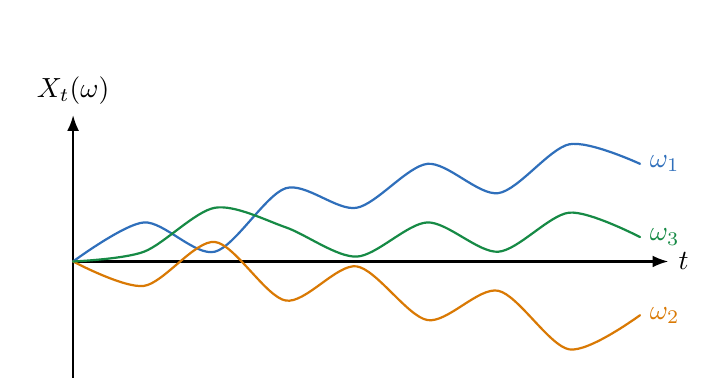
\begin{tikzpicture}[x=0.9cm,y=0.62cm,line cap=round]
\draw[diagramAxis] (0,0) -- (8.4,0) node[right] {$t$};
\draw[diagramAxis] (0,-2.6) -- (0,3.0) node[above] {$X_t(\omega)$};

\draw[diagramBlue,thick]
 plot[smooth] coordinates {(0,0) (1,0.8) (2,0.2) (3,1.5) (4,1.1)
 (5,2.0) (6,1.4) (7,2.4) (8,2.0)};
\draw[diagramOrange,thick]
 plot[smooth] coordinates {(0,0) (1,-0.5) (2,0.4) (3,-0.8) (4,-0.1)
 (5,-1.2) (6,-0.6) (7,-1.8) (8,-1.1)};
\draw[diagramGreen,thick]
 plot[smooth] coordinates {(0,0) (1,0.2) (2,1.1) (3,0.7) (4,0.1)
 (5,0.8) (6,0.2) (7,1.0) (8,0.5)};

\node[diagramBlue,right] at (8,2.0) {$\omega_1$};
\node[diagramOrange,right] at (8,-1.1) {$\omega_2$};
\node[diagramGreen,right] at (8,0.5) {$\omega_3$};
\end{tikzpicture}
\caption{Different outcomes generate different sample paths of the same
stochastic process.}
\label{fig:stochastic-process-sample-paths}
\end{figure}

\subsection{Stationarity}

A process \(X=(X_t)\) is \textbf{strictly stationary} if shifting the time
origin does not change any of its finite-dimensional distributions. Formally,
for every \(n\), every \(t_1,\ldots,t_n\), and every admissible shift \(h\),
\[
(X_{t_1+h},\ldots,X_{t_n+h})
\overset{d}{=}
(X_{t_1},\ldots,X_{t_n}).
\]
The process therefore has the same probabilistic behaviour after a time
shift.

A second-order process is \textbf{weakly stationary} if
\[
\mathbb{E}[X_t]=m
\]
is constant and
\[
\operatorname{Cov}(X_s,X_t)=C(t-s)
\]
depends only on the time lag.

\begin{quote}
\textbf{Important distinction.} Stationarity does not say that the future is
independent of the past. It says that the distributional rules are unchanged
by shifting time. Dependence may still be present.
\end{quote}

\subsection{Stationary and Independent Increments}

These are properties of changes in the process rather than of its absolute
level.

\paragraph{Stationary increments.}
The process has stationary increments if the distribution of
\[
X_{t+h}-X_t
\]
depends only on the interval length \(h\), not on the starting time \(t\).
When \(X_0=0\), this can be written
\[
X_{t+h}-X_t\overset{d}{=}X_h.
\]

\paragraph{Independent increments.}
For every sequence
\[
0\leq t_0<t_1<\cdots<t_n,
\]
the increments
\[
X_{t_1}-X_{t_0},
\quad
X_{t_2}-X_{t_1},
\quad\ldots\quad,
X_{t_n}-X_{t_{n-1}}
\]
are independent random variables. Thus changes over non-overlapping time
intervals do not influence one another.

For example, if \(t_1<t_2\leq t_3<t_4\), independent increments imply that
\[
X_{t_2}-X_{t_1}
\quad\text{and}\quad
X_{t_4}-X_{t_3}
\]
are independent.

\begin{center}
\begin{tabular}{L{0.28\textwidth}L{0.62\textwidth}}
\toprule
\textbf{Property} & \textbf{Meaning} \\
\midrule
Stationary process & The joint distribution of the levels is unchanged by a
common time shift. \\
Stationary increments & The distribution of a change depends only on the
length of its interval. \\
Independent increments & Changes over disjoint time intervals are
independent. \\
\bottomrule
\end{tabular}
\end{center}

Standard Brownian motion has stationary and independent increments, but it
is not itself stationary because
\(\operatorname{Var}(W_t)=t\) changes with time.

\subsection{Filtrations: Information Through Time}

A \textbf{filtration} is an increasing family of sub-sigma algebras
\[
(\mathcal{F}_t)_{t\in T}
\]
such that
\[
s\leq t
\quad\Longrightarrow\quad
\mathcal{F}_s\subseteq\mathcal{F}_t\subseteq\mathcal{F}.
\]
The sigma algebra \(\mathcal{F}_t\) represents all information available by
time \(t\). Information accumulates as time passes, so later sigma algebras
are larger. The quadruple
\[
(\Omega,\mathcal{F},(\mathcal{F}_t)_{t\in T},\mathbb{P})
\]
is called a \textbf{filtered probability space}.

\paragraph{Three-coin-flip example.}
Suppose a coin is flipped three times. Then
\[
\Omega
=\{HHH,HHT,HTH,HTT,THH,THT,TTH,TTT\}.
\]
Let \(C_k\) denote the result of flip \(k\), and define the natural
filtration
\[
\mathcal{F}_k=\sigma(C_1,\ldots,C_k).
\]

\begin{longtable}{@{}L{0.10\textwidth}L{0.35\textwidth}L{0.35\textwidth}L{0.09\textwidth}@{}}
\toprule
\textbf{Time} & \textbf{Information atoms} & \textbf{Interpretation} &
\textbf{Events} \\
\midrule
\(0\) & \(\Omega\) & No flip has been observed. Only impossible and certain
events are distinguishable. & \(2\) \\
\(1\) & \(A_H=\{HHH,HHT,HTH,HTT\}\),
\(A_T=\{THH,THT,TTH,TTT\}\) & The first flip is known. & \(2^2=4\) \\
\(2\) & \(A_{HH},A_{HT},A_{TH},A_{TT}\), according to the first two flips
& The first two flips are known. & \(2^4=16\) \\
\(3\) & The eight singleton outcomes & All three flips are known. &
\(2^8=256\) \\
\bottomrule
\end{longtable}

Each sigma algebra consists of every union of its information atoms. For
example,
\[
\mathcal{F}_0=\{\varnothing,\Omega\},
\qquad
\mathcal{F}_1=\{\varnothing,\Omega,A_H,A_T\}.
\]
If the realised sequence is \(HTH\), then the information narrows from
\(\Omega\) at time 0, to \(A_H\) after the first flip, to \(A_{HT}\) after
the second, and finally to the singleton \(\{HTH\}\).

\subsection{Adapted Processes}

A process \(X=(X_t)\) is \textbf{adapted} to the filtration
\((\mathcal{F}_t)\) if
\[
X_t\text{ is }\mathcal{F}_t\text{-measurable for every }t.
\]
Adaptedness means that the value \(X_t\) can be determined from information
available at time \(t\); it does not use future information.

For a stock-price process \(S_t\), adaptation means that events such as
\[
\{S_t\leq s\}
\]
belong to \(\mathcal{F}_t\). The market can observe the current and past
prices, but not future prices.

\subsection{Moment-Generating Functions}

For a real random variable \(X\), the \textbf{moment-generating function}
(MGF) is
\[
M_X(u)=\mathbb{E}\!\left[e^{uX}\right],
\]
for those real \(u\) at which the expectation is finite. Using
\[
e^{uX}=\sum_{k=0}^{\infty}\frac{u^kX^k}{k!},
\]
and interchanging expectation and summation when justified gives
\[
M_X(u)
=\sum_{k=0}^{\infty}\frac{u^k}{k!}\mathbb{E}[X^k].
\]
Hence, if the MGF exists on an open interval around zero,
\[
M_X^{(k)}(0)=\mathbb{E}[X^k].
\]
In particular,
\[
\mathbb{E}[X]=M_X'(0),
\qquad
\mathbb{E}[X^2]=M_X''(0),
\]
and
\[
\operatorname{Var}(X)
=M_X''(0)-\bigl(M_X'(0)\bigr)^2.
\]

The MGF need not exist away from zero for every distribution. For a Gaussian
random variable \(X\sim\mathcal{N}(\mu,\sigma^2)\), however,
\[
M_X(u)=\exp\!\left(\mu u+\frac{1}{2}\sigma^2u^2\right).
\]

\subsection{Characteristic Functions}

The \textbf{characteristic function} of a real random variable \(X\) is
\[
\varphi_X(u)
=\mathbb{E}\!\left[e^{iuX}\right],
\qquad u\in\mathbb{R},
\]
where \(i^2=-1\). Since \(|e^{iuX}|=1\), the characteristic function exists
for every real-valued random variable and every real \(u\), even when the MGF
does not exist. It is the Fourier transform of the probability distribution
of \(X\) and uniquely determines that distribution.

When the corresponding moments exist,
\[
\varphi_X^{(k)}(0)=i^k\mathbb{E}[X^k].
\]

\subsection{Gaussian Random Variables}

A Gaussian or normal random variable with mean \(\mu\) and variance
\(\sigma^2\) is written
\[
X\sim\mathcal{N}(\mu,\sigma^2)
\]
and has density
\[
f_X(x)
=\frac{1}{\sqrt{2\pi}\sigma}
\exp\!\left[-\frac{(x-\mu)^2}{2\sigma^2}\right].
\]
Its characteristic function is
\[
\boxed{
\varphi_X(u)
=\exp\!\left(i\mu u-\frac{1}{2}\sigma^2u^2\right)
}.
\]
For a standard normal variable \(Z\sim\mathcal{N}(0,1)\), this becomes
\[
\varphi_Z(u)=e^{-u^2/2}.
\]

\paragraph{Derivation.}
Substituting the Gaussian density into the definition gives
\[
\varphi_X(u)
=\frac{1}{\sqrt{2\pi}\sigma}
\int_{-\infty}^{\infty}
\exp\!\left(
iux-\frac{(x-\mu)^2}{2\sigma^2}
\right)\,dx.
\]
With \(x=\mu+\sigma z\),
\[
\varphi_X(u)
=e^{i\mu u}
\frac{1}{\sqrt{2\pi}}
\int_{-\infty}^{\infty}
\exp\!\left(-\frac{z^2}{2}+iu\sigma z\right)\,dz.
\]
Completing the square,
\[
-\frac{z^2}{2}+iu\sigma z
=-\frac{(z-iu\sigma)^2}{2}
-\frac{\sigma^2u^2}{2}.
\]
The remaining shifted Gaussian integral contributes 1 after normalization,
which yields
\[
\varphi_X(u)
=e^{i\mu u}e^{-\sigma^2u^2/2}.
\]

\subsection{Random Vectors and Covariance Matrices}

An \(n\)-dimensional random vector is
\[
\boldsymbol{X}
=(X_1,\ldots,X_n)^{\mathsf{T}}.
\]
Its mean is the vector
\[
\boldsymbol{\mu}
=\mathbb{E}[\boldsymbol{X}]
=\begin{pmatrix}
\mathbb{E}[X_1]\\
\vdots\\
\mathbb{E}[X_n]
\end{pmatrix},
\]
and its covariance matrix is
\[
\boldsymbol{\Sigma}
=\operatorname{Cov}(\boldsymbol{X}),
\qquad
\Sigma_{jk}
=\operatorname{Cov}(X_j,X_k)
=\mathbb{E}\!\left[(X_j-\mu_j)(X_k-\mu_k)\right].
\]
The matrix \(\boldsymbol{\Sigma}\) is symmetric and positive semidefinite.
Its diagonal entries are variances, while its off-diagonal entries measure
linear co-movement between components.

The multivariate characteristic function is
\[
\varphi_{\boldsymbol{X}}(\boldsymbol{u})
=\mathbb{E}\!\left[
e^{i\boldsymbol{u}^{\mathsf{T}}\boldsymbol{X}}
\right],
\qquad \boldsymbol{u}\in\mathbb{R}^n.
\]

\subsection{Gaussian Random Vectors}

A random vector \(\boldsymbol{X}\) is \textbf{jointly Gaussian} if every
linear combination
\[
\boldsymbol{u}^{\mathsf{T}}\boldsymbol{X}
\]
is a one-dimensional Gaussian random variable. If
\[
\boldsymbol{X}\sim\mathcal{N}_n
(\boldsymbol{\mu},\boldsymbol{\Sigma}),
\]
then
\[
\boldsymbol{u}^{\mathsf{T}}\boldsymbol{X}
\sim
\mathcal{N}\!\left(
\boldsymbol{u}^{\mathsf{T}}\boldsymbol{\mu},
\boldsymbol{u}^{\mathsf{T}}\boldsymbol{\Sigma}\boldsymbol{u}
\right),
\]
and
\[
\boxed{
\varphi_{\boldsymbol{X}}(\boldsymbol{u})
=\exp\!\left(
i\boldsymbol{u}^{\mathsf{T}}\boldsymbol{\mu}
-\frac{1}{2}
\boldsymbol{u}^{\mathsf{T}}
\boldsymbol{\Sigma}
\boldsymbol{u}
\right)
}.
\]

If \(X_1,\ldots,X_n\) are \textbf{independent} Gaussian variables, then the
vector is jointly Gaussian. Indeed,
\[
\begin{aligned}
\varphi_{\boldsymbol{X}}(\boldsymbol{u})
&=\mathbb{E}\!\left[
\prod_{k=1}^{n}e^{iu_kX_k}
\right]\\
&=\prod_{k=1}^{n}\mathbb{E}[e^{iu_kX_k}]\\
&=\exp\!\left(
i\sum_{k=1}^{n}u_k\mu_k
-\frac{1}{2}\sum_{k=1}^{n}u_k^2\sigma_k^2
\right).
\end{aligned}
\]

\begin{quote}
\colorbox{diagramOrange!12}{%
\parbox{\dimexpr\linewidth-2\fboxsep\relax}{%
\textbf{Important qualification.} Gaussian marginal distributions alone do
not guarantee that a vector is jointly Gaussian. Independence of Gaussian
components is sufficient, but without independence or the joint-Gaussian
assumption, every component may be normal while some linear combinations are
not.}}
\end{quote}

\subsection{Martingales}

Let \((\Omega,\mathcal{F},(\mathcal{F}_t),\mathbb{P})\) be a filtered
probability space. An adapted process \(X=(X_t)\) is a \textbf{martingale} if
\[
\mathbb{E}[|X_t|]<\infty
\]
for every \(t\), and, whenever \(s\leq t\),
\[
\boxed{
\mathbb{E}[X_t\mid\mathcal{F}_s]=X_s
}.
\]
Thus, given all information currently available, the conditional mean of a
future value is the present value. A martingale is often described as a
mathematical model of a fair game.

Suppose the observed value at time \(s\) is \(X_s=100\). Many future paths
may rise or fall, but their conditional average at a later time \(t\) is 100.
If new information arrives at a later time \(u\) and the realised value is
\(X_u=104\), then the updated conditional average of later values becomes
104. Conditional expectations change as the information set grows.

\paragraph{Random-walk example.}
Let
\[
X_n=\sum_{k=1}^{n}U_k,
\qquad
\mathbb{P}(U_k=1)=\mathbb{P}(U_k=-1)=\frac12,
\]
and let
\[
\mathcal{F}_n=\sigma(U_1,\ldots,U_n).
\]
Because \(U_{n+1}\) is independent of \(\mathcal{F}_n\) and has mean zero,
\[
\begin{aligned}
\mathbb{E}[X_{n+1}\mid\mathcal{F}_n]
&=\mathbb{E}[X_n+U_{n+1}\mid\mathcal{F}_n]\\
&=X_n+\mathbb{E}[U_{n+1}]\\
&=X_n.
\end{aligned}
\]
Therefore the simple symmetric random walk is a martingale with respect to
its natural filtration.

\paragraph{Submartingales and supermartingales.}
An integrable adapted process is a \textbf{submartingale} if
\[
\mathbb{E}[X_t\mid\mathcal{F}_s]\geq X_s,
\qquad s\leq t,
\]
and a \textbf{supermartingale} if
\[
\mathbb{E}[X_t\mid\mathcal{F}_s]\leq X_s.
\]
The terminology refers to conditional drift, not to monotone sample paths:
a submartingale can fall on individual paths, and a supermartingale can rise.

For a random walk with
\[
\mathbb{P}(U_k=1)=p,
\qquad
\mathbb{P}(U_k=-1)=1-p,
\]
the expected increment is \(2p-1\). The process is a submartingale when
\(p>1/2\), a martingale when \(p=1/2\), and a supermartingale when \(p<1/2\).

\paragraph{Connection to option pricing.}
Under a risk-neutral probability measure \(\mathbb{Q}\), it is generally the
\textbf{discounted} tradable asset price, rather than the undiscounted price,
that is modelled as a martingale. With a deterministic short rate \(r\),
\[
\widetilde{S}_t=e^{-rt}S_t
\]
satisfies
\[
\mathbb{E}^{\mathbb{Q}}
\!\left[\widetilde{S}_t\mid\mathcal{F}_s\right]
=\widetilde{S}_s,
\qquad s\leq t.
\]
Equivalently,
\[
S_s
=e^{-r(t-s)}
\mathbb{E}^{\mathbb{Q}}[S_t\mid\mathcal{F}_s].
\]
This conditional-expectation principle is central to no-arbitrage derivative
pricing.

\section{Concept Map}

\begin{longtable}{@{}L{0.25\textwidth}L{0.65\textwidth}@{}}
\toprule
\textbf{Concept} & \textbf{Role} \\
\midrule
Probability space & Specifies outcomes, measurable events, and their
probabilities. \\
Stochastic process & Provides a time-indexed family of random variables. \\
Sample path & Shows one realised evolution after an outcome \(\omega\) is
fixed. \\
Stationary increments & Makes the distribution of a change depend only on
elapsed time. \\
Independent increments & Separates randomness across disjoint intervals. \\
Filtration & Records the information available through time. \\
Adaptedness & Ensures the process uses no future information. \\
MGF and characteristic function & Encode a distribution and, when valid,
its moments. \\
Covariance matrix & Describes the scale and linear dependence of a random
vector. \\
Martingale & Expresses conditional fairness relative to a filtration. \\
\bottomrule
\end{longtable}

\chapter{Markov Chains}

Markov chains provide a middle ground between two extreme modelling choices.
An i.i.d. model assumes that successive observations are completely
independent, while a fully general time-series model may require the entire
past to predict the next observation. A Markov chain retains a local form of
dependence: the next state depends on the current state, but not on the full
history once the current state is known.

\section{Motivation}

\subsection{Why the Independence Assumption Can Fail}

A random variable represents a distribution of possible outcomes rather than
one deterministic number. Examples include
\[
X\sim\mathcal{N}(\mu,\sigma^2),
\qquad
Y\sim\operatorname{Bin}(n,p),
\qquad
Z\sim\operatorname{Bernoulli}(p).
\]
Repeatedly drawing from the same distribution is often modelled by an i.i.d.
sequence. This assumes both that the distribution remains unchanged and that
one observation contains no information about the next. In finance, these
assumptions can fail because return distributions drift, volatility changes,
and credit or market states persist through time.

\paragraph{An i.i.d. dice-roll portfolio.}
Suppose a portfolio value \(V_t\) is independently set each day by a fair die:
\[
\mathbb{P}(V_t=k)=\frac16,
\qquad k=1,\ldots,6.
\]
Then the values are time-invariant and independent. Knowing today's value
does not change tomorrow's distribution. This is mathematically convenient,
but it cannot express persistence or restrictions on how states evolve.

\paragraph{Loan-delinquency motivation.}
Consider four possible states for an individual loan:
\[
\mathcal{S}
=\{C,D_{30},D_{60},D_{90}\},
\]
where \(C\) denotes current, \(D_{30}\) denotes 30--59 days late,
\(D_{60}\) denotes 60--89 days late, and \(D_{90}\) denotes at least 90 days
late. If each month's state were drawn independently from a fixed categorical
distribution, a current loan could jump directly to \(D_{90}\) in one month.
That transition is inconsistent with the way delinquency ages.

The empirical proportion of delinquent loans,
\[
\widehat p
=\frac{\text{number of delinquent loans}}
       {\text{total number of loans}}
=\frac{1}{n}\sum_{\ell=1}^{n}
\mathbf{1}_{\{\text{loan }\ell\text{ is delinquent}\}},
\]
describes a cross-section at one time, but does not describe how individual
loans move between states. A transition model is needed.

\section{Core Structure and Probability Propagation}

\subsection{Definition and Markov Property}

Let \(X_0,X_1,\ldots\) take values in a finite state space
\(\mathcal{S}=\{1,\ldots,m\}\). The process is a \textbf{Markov chain} if,
for every admissible history,
\[
\boxed{
\mathbb{P}(X_{t+1}=j\mid X_t=i,X_{t-1}=i_{t-1},\ldots,X_0=i_0)
=\mathbb{P}(X_{t+1}=j\mid X_t=i)
}.
\]
This is the \textbf{Markov property}. It is often called memorylessness, but
the name should be interpreted carefully: the chain may be strongly
dependent through time. The statement is that the present state contains all
the historical information used by the model to predict the next state.

For the loan example,
\[
\begin{aligned}
&\mathbb{P}(X_{t+1}=D_{60}mid X_t=D_{30},X_{t-1}=C)\\
&\qquad=
\mathbb{P}(X_{t+1}=D_{60}\mid X_t=D_{30}).
\end{aligned}
\]

A chain is \textbf{time homogeneous} if the conditional probabilities do not
depend on the calendar time:
\[
\mathbb{P}(X_{t+1}=j\mid X_t=i)=p_{ij}
\quad\text{for every }t.
\]
Markov chains may also have countably infinite state spaces, but the notebook
and the applications below focus on finite, time-homogeneous chains.

\subsection{Transition Matrices}

The one-step transition probabilities are collected in the matrix
\[
P=(p_{ij})_{i,j=1}^{m},
\qquad
p_{ij}=\mathbb{P}(X_{t+1}=j\mid X_t=i).
\]
Every transition matrix is \textbf{row stochastic}:
\[
p_{ij}\geq0,
\qquad
\sum_{j=1}^{m}p_{ij}=1
\quad\text{for each }i.
\]
The row identifies the current state and the column identifies the next
state.

For the delinquency model, the structural zero pattern is
\[
P=
\begin{array}{c|cccc}
&C&D_{30}&D_{60}&D_{90}\\ \hline
C      &p_{11}&p_{12}&0&0\\
D_{30} &p_{21}&p_{22}&p_{23}&0\\
D_{60} &p_{31}&0&p_{33}&p_{34}\\
D_{90} &p_{41}&0&0&p_{44}
\end{array}.
\]
Missing arrows or zero entries encode transitions that the model declares
impossible in one step.

The numerical matrix used throughout the notebook is
\[
P=
\begin{pmatrix}
0.99&0.01&0&0\\
0.25&0.70&0.05&0\\
0.15&0&0.80&0.05\\
0.01&0&0&0.99
\end{pmatrix}.
\]

\begin{figure}[H]
\centering
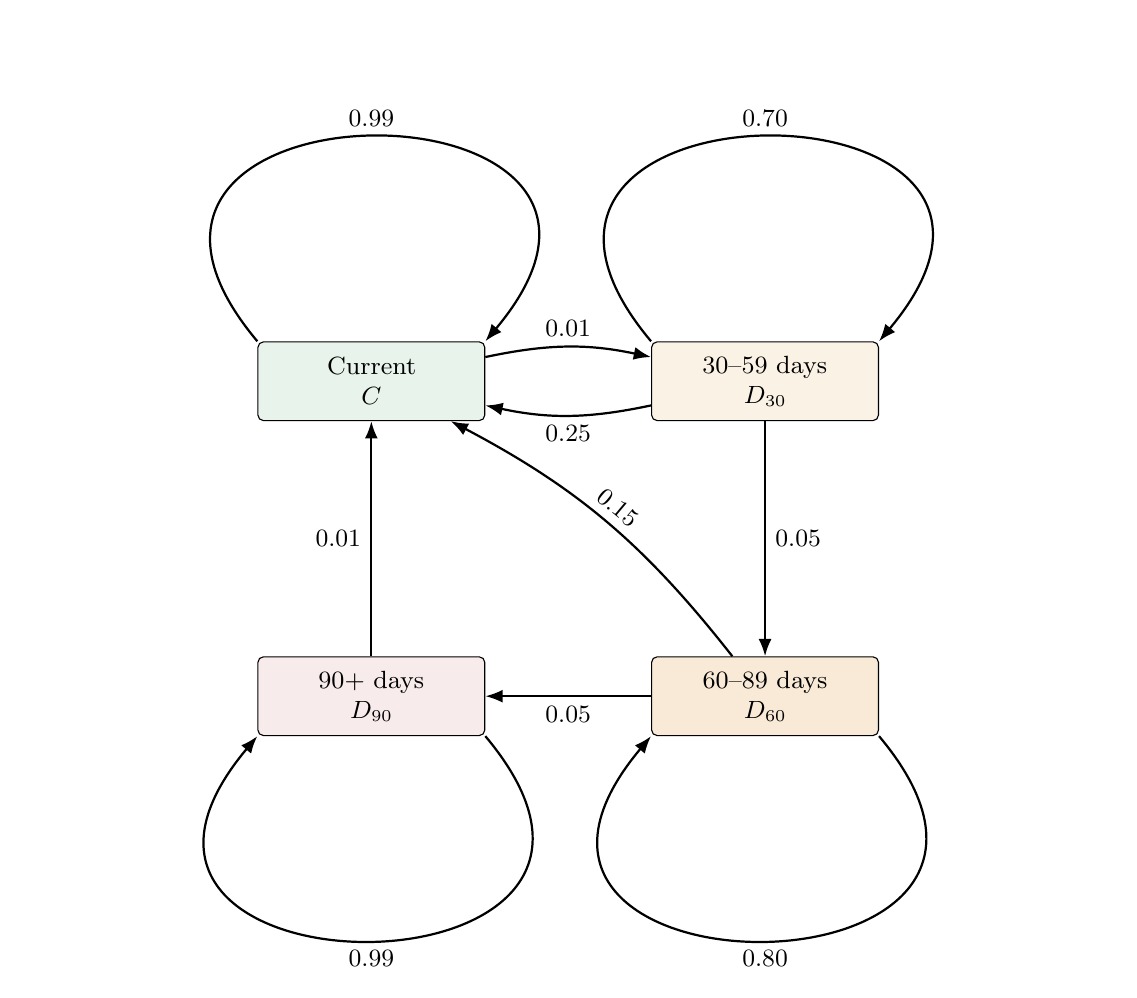
\begin{tikzpicture}[
    every node/.style={font=\small},
    state/.style={diagramBox,text width=2.6cm,minimum height=10mm},
    every edge/.style={diagramArrow}
]
\node[state,fill=diagramGreen!10] (c) at (0,2) {Current\\\(C\)};
\node[state,fill=diagramOrange!10] (d30) at (5,2) {30--59 days\\\(D_{30}\)};
\node[state,fill=diagramOrange!16] (d60) at (5,-2) {60--89 days\\\(D_{60}\)};
\node[state,fill=bearc!10] (d90) at (0,-2) {90+ days\\\(D_{90}\)};

\draw[diagramArrow] (c) to[bend left=12]
  node[above] {0.01} (d30);
\draw[diagramArrow] (d30) to[bend left=12]
  node[below] {0.25} (c);
\draw[diagramArrow] (d30) -- node[right] {0.05} (d60);
\draw[diagramArrow] (d60) -- node[below] {0.05} (d90);
\draw[diagramArrow] (d60) to[bend right=12]
  node[above,sloped] {0.15} (c);
\draw[diagramArrow] (d90) -- node[left] {0.01} (c);

\draw[diagramArrow] (c.north west)
  to[out=130,in=50,looseness=4] node[above] {0.99} (c.north east);
\draw[diagramArrow] (d30.north west)
  to[out=130,in=50,looseness=4] node[above] {0.70} (d30.north east);
\draw[diagramArrow] (d60.south east)
  to[out=310,in=230,looseness=4] node[below] {0.80} (d60.south west);
\draw[diagramArrow] (d90.south east)
  to[out=310,in=230,looseness=4] node[below] {0.99} (d90.south west);
\end{tikzpicture}
\caption{The loan-delinquency Markov chain. An omitted arrow represents a
zero one-step transition probability.}
\label{fig:loan-delinquency-markov-chain}
\end{figure}

The matrix describes the evolution of \textbf{each loan}, not the portfolio
as a single four-state object. The portfolio distribution is obtained by
aggregating the state probabilities of its individual loans.

\subsection{State-Distribution Vectors}

Let
\[
\boldsymbol{\pi}(t)
=\bigl(\pi_1(t),\ldots,\pi_m(t)\bigr)
\]
be a row vector, where
\[
\pi_i(t)=\mathbb{P}(X_t=i),
\qquad
\sum_{i=1}^{m}\pi_i(t)=1.
\]
The one-step evolution follows from the law of total probability:
\[
\pi_j(t+1)
=\sum_{i=1}^{m}\pi_i(t)p_{ij}.
\]
In matrix form,
\[
\boxed{
\boldsymbol{\pi}(t+1)=\boldsymbol{\pi}(t)P
}.
\]
For a portfolio of \(N\) statistically identical loans, the expected number
in state \(j\) at time \(t\) is
\[
\mathbb{E}[N_j(t)]=N\pi_j(t).
\]
This expectation formula does not require the loans to be mutually
independent, although independence strongly affects portfolio-level
uncertainty and confidence intervals.

\subsection{Chapman--Kolmogorov Equations}

Define the \(n\)-step transition probability
\[
p_{ij}^{(n)}
=\mathbb{P}(X_{t+n}=j\mid X_t=i).
\]
Conditioning on an intermediate state \(k\) gives the
\textbf{Chapman--Kolmogorov equation}
\[
\boxed{
p_{ij}^{(a+b)}
=\sum_{k=1}^{m}p_{ik}^{(a)}p_{kj}^{(b)}
}.
\]
Here \(m\) is the number of states, while \(a\) and \(b\) are elapsed numbers
of steps. In matrix form,
\[
P^{(a+b)}=P^{(a)}P^{(b)}.
\]
For a time-homogeneous chain, \(P^{(n)}=P^n\), and therefore
\[
\boldsymbol{\pi}(t)=\boldsymbol{\pi}(0)P^t.
\]

\subsection{Twelve-Month Loan Transition Probabilities}

For the loan matrix above, direct matrix multiplication gives
\[
P^{12}\approx
\begin{pmatrix}
0.95984&0.03168&0.00665&0.00183\\
0.89358&0.04109&0.03208&0.03324\\
0.69191&0.02031&0.07201&0.21576\\
0.11048&0.00272&0.00037&0.88644
\end{pmatrix}.
\]
Thus a currently performing loan has probability
\[
\mathbb{P}(X_{12}=D_{90}\mid X_0=C)
=(P^{12})_{C,D_{90}}
\approx0.001826,
\]
or approximately \(0.1826\%\), of being at least 90 days delinquent after
12 months under the model.

\begin{center}
\begin{tabular}{L{0.22\textwidth}rrrr}
\toprule
\textbf{Starting State} & \textbf{Current} & \textbf{30--59} &
\textbf{60--89} & \textbf{90+} \\
\midrule
Current & 95.98\% & 3.17\% & 0.66\% & 0.18\% \\
30--59 days & 89.36\% & 4.11\% & 3.21\% & 3.32\% \\
60--89 days & 69.19\% & 2.03\% & 7.20\% & 21.58\% \\
90+ days & 11.05\% & 0.27\% & 0.04\% & 88.64\% \\
\bottomrule
\end{tabular}
\end{center}

For the illustrative initial portfolio distribution
\[
\boldsymbol{\pi}(0)=(0.50,0.20,0,0.30),
\]
the genuine 12-month distribution is
\[
\boldsymbol{\pi}(12)
=\boldsymbol{\pi}(0)P^{12}
\approx(0.69178,0.02487,0.00985,0.27349).
\]
Therefore the expected 90+ delinquency proportion after 12 months is
approximately \(27.349\%\). For a portfolio of 1,000 loans, the corresponding
expected state counts are approximately
\[
(692,25,10,273).
\]

\begin{quote}
\colorbox{diagramOrange!12}{%
\parbox{\dimexpr\linewidth-2\fboxsep\relax}{%
\textbf{Notebook correction.} One notebook cell describes its result as a
12-month forecast but computes \(P^{10000}\). Its reported \(3.8462\%\) is
the long-run stationary 90+ proportion, not the 12-month proportion for the
stated initial distribution.}}
\end{quote}

\section{State Classification and Long-Run Behaviour}

\subsection{Accessibility, Communication, and Irreducibility}

A state \(j\) is \textbf{accessible} from state \(i\), written
\(i\to j\), if
\[
(P^n)_{ij}>0
\]
for some \(n\geq0\). States \(i\) and \(j\) \textbf{communicate} if
\(i\to j\) and \(j\to i\). Communication partitions the state space into
communication classes.

A chain is \textbf{irreducible} if every pair of states communicates. In an
irreducible finite chain, there is no permanently isolated regime: every
state can eventually reach every other state with positive probability.

For the loan matrix, the chain is irreducible. For example, \(C\to D_{30}\),
\(D_{30}\to D_{60}\), and \(D_{60}\to D_{90}\), while every delinquency
state can return to \(C\). Some transitions require several steps even though
their one-step probability is zero.

\subsection{Recurrence, Transience, and Absorption}

Starting from state \(i\), define the first return time
\[
T_i^+=\inf\{n\geq1:X_n=i\}.
\]
The state is \textbf{recurrent} if
\[
\mathbb{P}_i(T_i^+<\infty)=1,
\]
and \textbf{transient} if this probability is strictly less than 1. A
transient state has a positive probability of never being revisited after it
is left.

A state \(i\) is \textbf{absorbing} if
\[
p_{ii}=1.
\]
Once the chain enters an absorbing state, it can never leave. The loan matrix
has no absorbing state because every diagonal entry is less than 1, although
the states \(C\) and \(D_{90}\) are highly persistent. Because the displayed
chain is finite and irreducible, all four states are positive recurrent.

\subsection{Periodicity}

The period of state \(i\) is
\[
d(i)=\gcd\{n\geq1:(P^n)_{ii}>0\}.
\]
A state is \textbf{aperiodic} if \(d(i)=1\). In an irreducible chain all
states have the same period. A positive self-transition \(p_{ii}>0\) implies
aperiodicity for that state; therefore the loan chain is aperiodic because
every state has a self-loop.

\subsection{Stationary Distributions and Ergodicity}

A probability row vector \(\boldsymbol{\pi}^{*}\) is a
\textbf{stationary distribution} if
\[
\boxed{
\boldsymbol{\pi}^{*}P=\boldsymbol{\pi}^{*},
\qquad
\sum_{i=1}^{m}\pi_i^{*}=1
}.
\]
If \(X_0\sim\boldsymbol{\pi}^{*}\), then
\(X_t\sim\boldsymbol{\pi}^{*}\) at every later time.

For a finite irreducible and aperiodic chain, the stationary distribution is
unique and
\[
\boldsymbol{\pi}(0)P^t
\longrightarrow
\boldsymbol{\pi}^{*}
\qquad\text{as }t\to\infty
\]
for every initial distribution. This convergence property is commonly
called \textbf{ergodicity} in the finite-state setting.

Solving the stationary equations for the loan matrix gives
\[
\boldsymbol{\pi}^{*}
=\left(
\frac{120}{130},
\frac{4}{130},
\frac{1}{130},
\frac{5}{130}
\right)
\approx
(0.92308,0.03077,0.00769,0.03846).
\]
The long-run 90+ delinquency proportion is therefore \(3.8462\%\).

The evolution from the notebook's mixed initial distribution is summarized
below.

\begin{center}
\begin{tabular}{crrrr}
\toprule
\textbf{Month} & \textbf{Current} & \textbf{30--59} &
\textbf{60--89} & \textbf{90+} \\
\midrule
0 & 50.000\% & 20.000\% & 0.000\% & 30.000\% \\
1 & 54.800\% & 14.500\% & 1.000\% & 29.700\% \\
2 & 58.324\% & 10.698\% & 1.525\% & 29.453\% \\
12 & 69.178\% & 2.487\% & 0.985\% & 27.349\% \\
50 & 77.115\% & 2.552\% & 0.631\% & 19.701\% \\
\(\infty\) & 92.308\% & 3.077\% & 0.769\% & 3.846\% \\
\bottomrule
\end{tabular}
\end{center}

The convergence is slow because \(D_{90}\) has a \(99\%\) monthly
self-transition probability. Thus 50 months illustrates movement toward the
steady state, but does not yet closely approximate it.

\begin{quote}
\colorbox{diagramOrange!12}{%
\parbox{\dimexpr\linewidth-2\fboxsep\relax}{%
\textbf{Steady-state warning.} The limiting distribution is meaningful only
if the transition mechanism remains stable. Economic cycles, seasonality,
policy changes, underwriting changes, and external shocks can make the true
transition matrix vary through time.}}
\end{quote}

\section{Model Design and Estimation}

\subsection{Choosing States in Quantitative Finance}

State definitions are problem dependent. Common choices include
\begin{itemize}
    \item \textbf{volatility regimes:} low, medium, and high, using a measure
    such as the VIX or realised volatility;
    \item \textbf{market trends:} bullish, bearish, and sideways, using index
    returns or trend indicators;
    \item \textbf{liquidity regimes:} tight, normal, and wide spreads, using
    quoted or effective bid--ask spreads;
    \item \textbf{credit states:} current and progressively older
    delinquency buckets.
\end{itemize}

Thresholds should be chosen before estimating transitions, or selected using
a properly separated training sample. Poor thresholds can discard important
information or create states with too few observed transitions.

\subsection{Maximum Likelihood Estimation: General Idea}

Maximum likelihood estimation chooses the parameter value under which the
observed data have the greatest probability or density. For example, if
\(Y_1,\ldots,Y_n\) are modelled as i.i.d.
\(\mathcal{N}(\mu,\sigma^2)\), then maximizing the Gaussian likelihood gives
\[
\widehat\mu
=\frac1n\sum_{k=1}^{n}Y_k,
\qquad
\widehat\sigma^2
=\frac1n\sum_{k=1}^{n}(Y_k-\widehat\mu)^2.
\]
As more representative observations become available, these estimates
typically stabilize near the data-generating parameters. Early estimates can
be volatile because they are based on small samples.

The same principle estimates a Markov transition matrix: instead of fitting
the parameters of one density, we fit every row of conditional transition
probabilities.

\subsection{Deriving the Markov-Chain MLE}

Suppose the observed state sequence is
\[
x_0,x_1,\ldots,x_T,
\]
and let \(\nu_i=\mathbb{P}(X_0=i)\) be the initial distribution. Under the
time-homogeneous Markov model, the likelihood is
\[
L(P)
=\nu_{x_0}
\prod_{t=0}^{T-1}p_{x_t x_{t+1}}.
\]
Define the transition counts
\[
n_{ij}
=\sum_{t=0}^{T-1}
\mathbf{1}_{\{x_t=i,x_{t+1}=j\}},
\qquad
n_i=\sum_{j=1}^{m}n_{ij}.
\]
Then
\[
L(P)
=\nu_{x_0}
\prod_{i=1}^{m}\prod_{j=1}^{m}p_{ij}^{n_{ij}},
\]
and, ignoring the initial term when it does not involve \(P\),
\[
\ell(P)
=\log L(P)
=\text{constant}
+\sum_{i=1}^{m}\sum_{j=1}^{m}n_{ij}\log p_{ij}.
\]

Each row is maximized subject to
\[
\sum_{j=1}^{m}p_{ij}=1,
\qquad
p_{ij}\geq0.
\]
For row \(i\), use the Lagrangian
\[
\mathcal{L}_i
=\sum_{j=1}^{m}n_{ij}\log p_{ij}
+\lambda_i\left(1-\sum_{j=1}^{m}p_{ij}\right).
\]
The first-order condition is
\[
\frac{\partial\mathcal{L}_i}{\partial p_{ij}}
=\frac{n_{ij}}{p_{ij}}-\lambda_i=0,
\]
so \(p_{ij}=n_{ij}/\lambda_i\). Summing over \(j\) yields
\(\lambda_i=n_i\), and therefore
\[
\boxed{
\widehat p_{ij}
=\frac{n_{ij}}{n_i}
=\frac{\text{observed transitions }i\to j}
       {\text{all observed departures from }i}
}.
\]
The MLE is simply the observed transition frequency within each row. If
\(n_i=0\), that row cannot be estimated from the data without additional
structure or smoothing.

For multiple loan histories, the counts \(n_{ij}\) are aggregated across all
loans and all adjacent observation times. The chain is fitted to each loan's
state transitions, not directly to the aggregate portfolio proportions.

\subsection{Loan-Portfolio MLE Example}

The notebook generates 1,000 loan histories over 12 months using the matrix
\[
P=
\begin{pmatrix}
0.99&0.01&0&0\\
0.25&0.70&0.05&0\\
0.15&0&0.80&0.05\\
0.01&0&0&0.99
\end{pmatrix}
\]
and an initial distribution
\[
(0.85,0.08,0.05,0.02).
\]
One simulated cross-section contains 865 current loans, 67 loans 30--59 days
late, 46 loans 60--89 days late, and 22 loans at least 90 days late. Sampling
variation explains why these counts are not exactly equal to their expected
values \((850,80,50,20)\).

Aggregating observed transitions gives the MLE
\[
\widehat P\approx
\begin{pmatrix}
0.99198&0.00802&0&0\\
0.23325&0.71712&0.04963&0\\
0.15504&0&0.77132&0.07364\\
0.00545&0&0&0.99455
\end{pmatrix}.
\]
The estimates are close to the generating matrix. Rows or transitions with
fewer observations show greater sampling error; for example, the estimated
\(D_{60}\to D_{90}\) probability differs more noticeably from its true value
than the frequently observed current-state probabilities.

\subsection{Assumptions Behind the Estimator}

The interpretation and large-sample reliability of \(\widehat P\) depend on
several assumptions.

\begin{enumerate}
    \item \textbf{Markov property.} The current state contains all past
    information relevant to the next transition.

    \item \textbf{Time homogeneity.} The matrix \(P\) is constant across the
    sample and forecast horizon.

    \item \textbf{Sufficient state visitation.} Every row of interest has
    enough departures, and rare transitions are observed often enough to be
    estimated.

    \item \textbf{Ergodicity for one long history.} The chain must explore
    its relevant states so empirical transition frequencies converge to
    stable probabilities.

    \item \textbf{Cross-sectional independence or an appropriate dependence
    model.} Treating different loans as independent ignores shared exposure
    to unemployment, interest rates, geography, underwriting standards, and
    other macroeconomic shocks.
\end{enumerate}

Time homogeneity and cross-loan independence are often the most questionable
assumptions in credit applications. Violating them can make standard errors
too small and long-horizon forecasts misleading.

\subsection{Large-Sample Properties of the MLE}

Under suitable regularity, identifiability, and ergodicity conditions, the
transition-frequency estimator has the following properties.

\begin{itemize}
    \item \textbf{Consistency:} \(\widehat p_{ij}\to p_{ij}\) as the number
    of observed departures from state \(i\) grows.

    \item \textbf{Asymptotic normality:} conditional on \(n_i\), row \(i\)
    behaves like a multinomial estimate. Writing
    \(\boldsymbol{p}_i=(p_{i1},\ldots,p_{im})^{\mathsf T}\),
    \[
    \sqrt{n_i}
    (\widehat{\boldsymbol{p}}_i-\boldsymbol{p}_i)
    \xrightarrow{d}
    \mathcal{N}\!\left(
    \boldsymbol{0},
    \operatorname{diag}(\boldsymbol{p}_i)
    -\boldsymbol{p}_i\boldsymbol{p}_i^{\mathsf T}
    \right).
    \]

    \item \textbf{Asymptotic efficiency:} under standard conditions, the MLE
    achieves the usual information-bound efficiency within the specified
    model.

    \item \textbf{Invariance:} if \(g(P)\) is a function of the transition
    parameters, its MLE is \(g(\widehat P)\). For example, an estimated
    \(n\)-step matrix is \(\widehat P^{,n}\).
\end{itemize}

The law of large numbers explains why empirical probabilities tend to move
toward their true values as the data set grows. It does not guarantee that a
misspecified Markov model converges to the real economic mechanism.

\begin{quote}
\textbf{MLE versus maximum entropy.} Maximum likelihood and maximum entropy
are distinct principles. The MLE maximizes the likelihood of the observed
data. It is not generally a maximum-entropy estimator unless a separate
entropy argument and appropriate constraints establish that connection.
\end{quote}

\section{Limitations and Extensions}

The Markov assumption is a substantial improvement over unconditional
independence, but it remains a simplification. Important limitations include
\begin{itemize}
    \item dependence on events further in the past than the current state;
    \item transition probabilities that vary with economic conditions;
    \item common shocks that couple many loans or assets;
    \item imperfect, noisy, or arbitrarily discretized state definitions;
    \item unobserved regimes that influence the observed process.
\end{itemize}

Natural extensions include higher-order Markov chains, non-homogeneous
transition matrices, covariate-dependent transition models, regime-switching
models, and hidden Markov models. In quantitative finance, Markov chains are
often the first step toward models of volatility regimes, liquidity regimes,
credit migration, and latent market states.

\begin{quote}
\colorbox{diagramGreen!10}{%
\parbox{\dimexpr\linewidth-2\fboxsep\relax}{%
\textbf{Core modelling lesson.} Full independence is frequently too strong.
Markov chains replace it with local conditional dependence, enabling
probabilities and expectations to be propagated with a transition matrix.
The resulting model is useful only to the extent that its states, transition
rules, and stability assumptions reflect the real system.}}
\end{quote}

\medskip
\hrule
\medskip

\chapter{Random Walk}

A random walk is a concrete discrete-time stochastic process and, when its
current position is taken as the state, a Markov chain. The simple symmetric
case below turns the preceding abstract ideas into explicit paths,
probabilities, and barrier calculations before leading naturally to Brownian
motion.

\section{Simple Symmetric Random Walk}

\subsection{Definition and Rule}

A \textbf{simple symmetric random walk} is one of the simplest stochastic
processes. At every discrete time step, there is:
\begin{itemize}
    \item a \(50\%\) probability of moving \(+1\), one unit to the right;
    \item a \(50\%\) probability of moving \(-1\), one unit to the left.
\end{itemize}

\paragraph{Update rule.}
\[
x(n+1)=x(n)\pm 1.
\]
Each outcome, \(+1\) or \(-1\), is equally likely; this is why the walk is
called symmetric.

\subsection{Coin-Flip Analogy}

\begin{center}
\begin{tabular}{cc}
\toprule
\textbf{Coin-Flip Outcome} & \textbf{Movement} \\
\midrule
Heads & Move \(+1\) \\
Tails & Move \(-1\) \\
\bottomrule
\end{tabular}
\end{center}

\subsection{The Growing Tree of Possible Positions}

\begin{center}
\begin{tabular}{cL{0.55\textwidth}}
\toprule
\textbf{Time \(n\)} & \textbf{Possible Positions} \\
\midrule
0 & \(\{0\}\) \\
1 & \(\{-1,+1\}\) \\
2 & \(\{-2,0,+2\}\) \\
3 & \(\{-3,-1,+1,+3\}\) \\
\bottomrule
\end{tabular}
\end{center}

\begin{figure}[H]
\centering
\begin{tikzpicture}[
    level distance=10mm,
    level 1/.style={sibling distance=58mm},
    level 2/.style={sibling distance=29mm},
    level 3/.style={sibling distance=14mm},
    every node/.style={font=\small},
    edge from parent/.style={draw,diagramBlue,thick}
]
\node {$0$}
 child {node {$-1$}
   child {node {$-2$}
     child {node {$-3$}}
     child {node {$-1$}}}
   child {node {$0$}
     child {node {$-1$}}
     child {node {$+1$}}}}
 child {node {$+1$}
   child {node {$0$}
     child {node {$-1$}}
     child {node {$+1$}}}
   child {node {$+2$}
     child {node {$+1$}}
     child {node {$+3$}}}};
\end{tikzpicture}
\caption{The first three steps of a simple symmetric random walk.}
\label{fig:symmetric-random-walk-tree}
\end{figure}

\begin{quote}
\colorbox{diagramOrange!12}{%
\parbox{\dimexpr\linewidth-2\fboxsep\relax}{%
\textbf{Key intuition.} As time progresses, the number of possible paths and
reachable positions increases, making the path increasingly unpredictable
even though the movement rule remains simple. In the limit of many suitably
scaled small steps, this behaviour leads to Brownian motion.}}
\end{quote}

\section{Counting Random-Walk Paths}

The combinatorial approach to random walks treats every sequence of upward
and downward steps as a path. This viewpoint is especially useful because,
when the steps are independent and equally likely, calculating a probability
reduces to counting the paths in the corresponding event.

\subsection{Paths Between Two Space--Time Points}

Let
\[
\alpha=(m,p),
\qquad
\beta=(n,q),
\qquad m<n,
\]
be two points in the space--time plane. A random-walk path from \(\alpha\) to
\(\beta\) is a function
\[
\pi:\{m,m+1,\ldots,n\}\longrightarrow\mathbb{Z}
\]
such that
\[
\pi(m)=p,
\qquad
\pi(n)=q,
\qquad
|\pi(k+1)-\pi(k)|=1.
\]
Thus each step changes the position by exactly one unit. Denote the set of
all such paths by
\[
\operatorname{PATH}(\alpha,\beta).
\]

For paths starting at the origin, define
\[
N_{n,x}
:=
\left|
\operatorname{PATH}\bigl((0,0),(n,x)\bigr)
\right|.
\]

\subsection{Total Number of Paths}

At each of \(n\) time steps there are two possible moves, \(+1\) or \(-1\).
Consequently, the total number of length-\(n\) paths starting at the origin is
\[
2^n.
\]
Under the simple symmetric random-walk model, every one of these paths has
probability \(2^{-n}\).

\subsection{Number of Paths to a Fixed Endpoint}

Suppose a path reaches position \(x\) after \(n\) steps. If \(u\) is the
number of upward steps and \(d\) the number of downward steps, then
\[
u+d=n,
\qquad
u-d=x.
\]
Solving these equations gives
\[
u=\frac{n+x}{2},
\qquad
d=\frac{n-x}{2}.
\]
The path is determined once the \(u\) time indices containing upward steps
are selected. Hence
\[
N_{n,x}
=
\begin{cases}
\displaystyle \binom{n}{(n+x)/2},
& |x|\leq n\text{ and }n+x\text{ is even},\\[8pt]
0,
& \text{otherwise}.
\end{cases}
\]

The parity condition is important: after an even number of steps the walk
can reach only even positions, while after an odd number of steps it can
reach only odd positions. Dividing the path count by \(2^n\) gives the
endpoint distribution
\[
\boxed{
\mathbb{P}(X_n=x)
=2^{-n}N_{n,x}
=2^{-n}\binom{n}{(n+x)/2}
},
\]
whenever the endpoint is reachable.

\paragraph{Example: returning to the origin after ten steps.}
To finish at the starting position, the path must contain five upward and
five downward steps. Therefore
\[
\mathbb{P}(X_{10}=0)
=\frac{N_{10,0}}{2^{10}}
=\frac{\binom{10}{5}}{2^{10}}
=\frac{252}{1024}
=\frac{63}{256}
\approx0.2461.
\]

\subsection{A Useful Recursion}

Every path ending at \((n,x)\) must arrive on its final step either from
\((n-1,x-1)\) or from \((n-1,x+1)\). The two possibilities are disjoint, so
\[
N_{n,x}=N_{n-1,x-1}+N_{n-1,x+1},
\qquad N_{0,0}=1.
\]
This recurrence is the same addition rule that generates Pascal's triangle,
which explains the appearance of binomial coefficients in the endpoint
formula.

\subsection{Translation Invariance}

Shifting a path horizontally or vertically does not change its pattern of
upward and downward steps. Therefore
\[
\left|
\operatorname{PATH}\bigl((a,p),(b,q)\bigr)
\right|
=N_{b-a,q-p}.
\]
Only the elapsed time \(b-a\) and the net displacement \(q-p\) matter.

\paragraph{Example.}
A path from \((2,3)\) to \((15,2)\) has length \(13\) and displacement
\(-1\). Translating its starting point to the origin gives
\[
\left|
\operatorname{PATH}\bigl((2,3),(15,2)\bigr)
\right|
=N_{13,-1}
=\binom{13}{6}
=1716.
\]

\section{Return Probabilities}

A simple symmetric random walk can return to the origin only after an even
number of steps. At time \(2n\), exactly \(n\) steps must be upward and \(n\)
must be downward, so
\[
\boxed{
\mathbb{P}(X_{2n}=0)
=\frac{\binom{2n}{n}}{2^{2n}}
}.
\]
For \(n=5\), this reproduces the ten-step probability \(63/256\). Stirling's
approximation further gives
\[
\mathbb{P}(X_{2n}=0)
\sim\frac{1}{\sqrt{\pi n}}
\qquad\text{as }n\to\infty.
\]
Thus the probability of being at the origin at one particular late time
decreases to zero, but only at the relatively slow rate \(n^{-1/2}\).

\section{The Reflection Principle}

Path counting becomes more subtle when a path is required to touch, cross,
or avoid a barrier. The reflection principle converts such a constrained
count into an unconstrained endpoint count.

Let \(L\) be the horizontal line at integer height \(h\), and let
\[
\alpha=(m,p),
\qquad
\beta=(n,q),
\]
lie strictly on the same side of \(L\). Reflect \(\alpha\) across \(L\) to
obtain
\[
\alpha'=(m,2h-p).
\]

\begin{quote}
\colorbox{diagramBlue!8}{%
\parbox{\dimexpr\linewidth-2\fboxsep\relax}{%
\textbf{Reflection principle.} The number of paths from \(\alpha\) to
\(\beta\) that touch or cross \(L\) is equal to the total number of
unrestricted paths from the reflected point \(\alpha'\) to \(\beta\):
\[
\#\{\alpha\to\beta\text{ paths meeting }L\}
=\left|\operatorname{PATH}(\alpha',\beta)\right|.
\]}}
\end{quote}

Using translation invariance, this count can be written explicitly as
\[
\left|\operatorname{PATH}(\alpha',\beta)\right|
=N_{n-m,q-(2h-p)}
=N_{n-m,q-2h+p}.
\]

\begin{figure}[H]
\centering
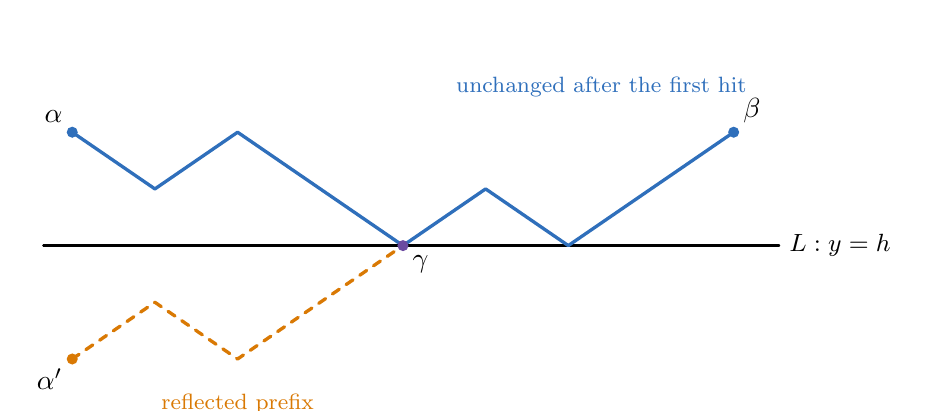
\begin{tikzpicture}[x=1.05cm,y=0.72cm,line cap=round,line join=round]
\draw[black,thick] (-0.35,0) -- (8.55,0)
  node[right,font=\small] {$L:y=h$};

\draw[diagramBlue,very thick]
  plot coordinates {(0,2) (1,1) (2,2) (3,1) (4,0) (5,1) (6,0) (7,1) (8,2)};
\draw[diagramOrange,very thick,dashed]
  plot coordinates {(0,-2) (1,-1) (2,-2) (3,-1) (4,0)};

\fill[diagramBlue] (0,2) circle (2pt)
  node[above left,black] {$\alpha$};
\fill[diagramOrange] (0,-2) circle (2pt)
  node[below left,black] {$\alpha'$};
\fill[diagramPurple] (4,0) circle (2pt)
  node[below right,black] {$\gamma$};
\fill[diagramBlue] (8,2) circle (2pt)
  node[above right,black] {$\beta$};

\node[font=\footnotesize,diagramOrange,align=center] at (2,-2.8)
  {reflected prefix};
\node[font=\footnotesize,diagramBlue,align=center] at (6.4,2.8)
  {unchanged after the first hit};
\end{tikzpicture}
\caption{Reflecting the path up to its first meeting point \(\gamma\) with
the barrier produces a path from \(\alpha'\) to \(\beta\).}
\label{fig:random-walk-reflection-principle}
\end{figure}

\subsection{Why the Reflection Principle Works}

Let \(\mathcal{S}\) be the set of paths from \(\alpha\) to \(\beta\) that
meet \(L\). For any \(\pi\in\mathcal{S}\), let
\[
\tau=\min\{k:\pi(k)=h\}
\]
be the first time the path meets the barrier. Define a new path by reflecting
the part before this first meeting:
\[
(f\pi)(k)
=
\begin{cases}
2h-\pi(k), & m\leq k\leq\tau,\\
\pi(k), & \tau\leq k\leq n.
\end{cases}
\]
The transformed path starts at \(\alpha'\), passes through the same first
meeting point \(\gamma=(\tau,h)\), and then follows the original path to
\(\beta\).

This construction is a bijection:
\begin{enumerate}
    \item Every constrained path produces a path from \(\alpha'\) to
    \(\beta\).
    \item Since \(\alpha'\) and \(\beta\) lie on opposite sides of \(L\),
    every path between them must meet \(L\).
    \item Reflecting the prefix of that path up to its first meeting with
    \(L\) recovers the unique original path.
\end{enumerate}
Therefore the constrained and reflected path sets have the same size.

\subsection{Counting Paths That Avoid a Barrier}

The total number of paths from \(\alpha=(m,p)\) to \(\beta=(n,q)\) is
\(N_{n-m,q-p}\). Subtracting the number that meet \(L\) gives
\[
\boxed{
\#\{\alpha\to\beta\text{ paths avoiding }L\}
=N_{n-m,q-p}-N_{n-m,q-2h+p}
}.
\]
This formula is the basic tool for questions about positivity, maximum
levels, and first-passage events.

\paragraph{Example: paths that remain strictly positive.}
Count the ten-step paths from \((0,0)\) to \((10,4)\) that satisfy
\(X_k>0\) for every \(k=1,\ldots,10\). The first step must be upward, so the
problem reduces to paths from \((1,1)\) to \((10,4)\) that avoid the line
\(L:y=0\). Thus
\[
\begin{aligned}
\#\{\text{strictly positive paths ending at }4\}
&=N_{9,3}-N_{9,5}\\
&=\binom{9}{6}-\binom{9}{7}\\
&=84-36\\
&=48.
\end{aligned}
\]
Since there are \(2^{10}\) total ten-step paths, the corresponding
unconditional probability is
\[
\frac{48}{2^{10}}=\frac{3}{64}.
\]

\section{Interpretation and Limitations in Finance}

A scaled random walk can be used as a first model of price changes:
\[
S_n=S_0+aX_n,
\]
where \(a\) is the monetary size of one price movement. The model captures
the idea that short-term changes are uncertain and that many possible price
paths may emerge from the same initial value. It also gives exact formulas
for endpoint probabilities and barrier events.

However, the simple symmetric model is not a realistic complete model of an
asset price:
\begin{itemize}
    \item it assumes equal probabilities of upward and downward moves;
    \item it assumes independent increments of constant size;
    \item it permits negative values when applied directly to prices;
    \item it does not account for changing volatility, jumps, or market
    microstructure.
\end{itemize}
These limitations motivate the continuous-time Brownian-motion and geometric
Brownian-motion models developed in the following sections.

\section{Random Walk as the Discrete Precursor to Brownian Motion}

Let \(\boldsymbol{X}=(X_0,X_1,X_2,\ldots)\) be the symmetric simple random
walk defined by
\[
X_n=\sum_{i=1}^{n}U_i,
\]
where \(\boldsymbol{U}=(U_1,U_2,\ldots)\) is a sequence of independent random
variables satisfying
\[
\mathbb{P}(U_i=1)=\mathbb{P}(U_i=-1)=\frac{1}{2}
\qquad\text{for every }i.
\]

\paragraph{Key statistical properties.}
\[
\mathbb{E}[X_n]=0,
\qquad
\operatorname{Var}(X_n)=n.
\]
Because \(X\) is the partial-sum process of an i.i.d. sequence, it has
\textbf{stationary, independent increments}, although only in discrete time.

\paragraph{Central Limit Theorem connection.}
\[
\frac{X_n}{\sqrt{n}}
\xrightarrow{d}
\mathcal{N}(0,1)
\qquad\text{as }n\to\infty.
\]

\paragraph{Constructing a continuous-time process.}
For \(h,d\in(0,\infty)\), define the continuous-time jump process
\[
X_{h,d}(t)=dX_{\lfloor t/h\rfloor}.
\]
Its jumps occur at \(\{0,h,2h,\ldots\}\), and every jump has size \(\pm d\).

We want to let \(h\downarrow0\), producing smaller time steps, and
\(d\downarrow0\), producing smaller spatial jumps, simultaneously. These
limits cannot be chosen arbitrarily because
\[
\mathbb{E}[X_{h,d}(t)]=0,
\qquad
\operatorname{Var}[X_{h,d}(t)]
=d^2\left\lfloor\frac{t}{h}\right\rfloor
\approx\frac{d^2t}{h}.
\]

\paragraph{The critical scaling.}
If \(d=\sqrt{h}\), the Central Limit Theorem implies that the distribution of
\(X_{h,d}(t)\) converges to a normal distribution with mean 0 and variance
\(t\) as \(h\downarrow0\):
\[
\boxed{
d=\sqrt{h}
\quad\Longrightarrow\quad
X_{h,d}(t)\xrightarrow{d}\mathcal{N}(0,t)
}.
\]

\begin{quote}
\colorbox{diagramGreen!10}{%
\parbox{\dimexpr\linewidth-2\fboxsep\relax}{%
\textbf{The mathematical bridge.} When the random walk's spatial step is the
square root of its time step, the scaled discrete process converges to
standard Brownian motion. Its limiting paths are continuous and appear
smooth at a distance, but are almost surely nowhere differentiable.}}
\end{quote}

\chapter{Derivatives}

\section{Brownian Motion}
\section{Modelling Stock Price}
\section{Itô's Lemma and Girsanov's Theorem}
\section{Factors Affecting Option Prices}
\section{Black--Scholes}
\section{Deriving the Black--Scholes Equation}
\section{Options Pricing}
\section{Binomial Model}
\section{Option Greeks}

\chapter{Machine Learning in Financial Markets}

\section{Sentiment Analysis: Opinion Mining}
\section{Research Papers}
\section{Datasets for Self-Practice}
\section{Time Series Analysis: Handling Volatility}
\section{Sequence-to-Sequence Modelling in Finance}



\end{document}